\documentclass[reqno]{amsart}

\usepackage[margin=2.5cm]{geometry}
\usepackage[pdftex]{graphicx}
\usepackage[utf8]{inputenc}
\usepackage[T1]{fontenc}
\usepackage{textcomp}
\usepackage{babel}
\usepackage{amsmath, amssymb, amsthm, amscd}
\usepackage[colorlinks=true,linkcolor=blue]{hyperref}
\usepackage{float}
\usepackage{mathrsfs}
\usepackage{todonotes}
%\usepackage{enumitem}
%% for identity function 1:
\usepackage{bbm}
%%For category theory diagrams:
\usepackage{tikz-cd}
%%For code (e.g. python) in latex:
%\usepackage{listings}
%
%Usage: 
%\begin{lstlisting}[language=Python]
%\end{lstlisting}

\newcommand{\incfig}[2][1]{%
\def\svgwidth{#1\columnwidth}
\import{./figures/}{#2.pdf_tex}
}


\theoremstyle{plain}% default
\newtheorem{theorem}{Theorem}[section]
\newtheorem{lemma}[theorem]{Lemma}
\newtheorem{proposition}[theorem]{Proposition}
\newtheorem{corollary}[theorem]{Corollary}


\theoremstyle{definition}
\newtheorem{definition}[theorem]{Definition}
\newtheorem{example}[theorem]{Example}
\newtheorem{exercise}[theorem]{Exercise}
\newtheorem{problem}[theorem]{Problem}


\theoremstyle{remark}
\newtheorem*{remark}{Remark}
\newtheorem*{note}{Note}
\newtheorem*{solution}{Solution}






% figure support
\usepackage{import}
\usepackage{xifthen}
\pdfminorversion=7
\usepackage{pdfpages}
\usepackage{transparent}

\pdfsuppresswarningpagegroup=1

\setlength\parindent{0pt}

\newcommand{\qedwhite}{\hfill \ensuremath{\Box}}

%Inequalities
\newcommand{\cycsum}{\sum_{\mathrm{cyc}}}
\newcommand{\symsum}{\sum_{\mathrm{sym}}}
\newcommand{\cycprod}{\prod_{\mathrm{cyc}}}
\newcommand{\symprod}{\prod_{\mathrm{sym}}}

%Linear Algebra

\DeclareMathOperator{\Span}{span}
\DeclareMathOperator{\Ima}{Im}
\DeclareMathOperator{\diag}{diag}
\DeclareMathOperator{\Ker}{Ker}
\DeclareMathOperator{\ob}{ob}
\DeclareMathOperator{\sk}{sk}
\DeclareMathOperator{\Vect}{Vect}
\DeclareMathOperator{\Set}{Set}
\DeclareMathOperator{\Group}{Group}
\DeclareMathOperator{\Ring}{Ring}
\DeclareMathOperator{\Ab}{Ab}
\DeclareMathOperator{\Top}{Top}
\DeclareMathOperator{\hTop}{hTop}
\DeclareMathOperator{\Htpy}{Htpy}
\DeclareMathOperator{\Cat}{Cat}
\DeclareMathOperator{\CAT}{CAT}
\DeclareMathOperator{\Cone}{Cone}
\DeclareMathOperator{\dom}{dom}
\DeclareMathOperator{\cod}{cod}
\DeclareMathOperator{\Aut}{Aut}
\DeclareMathOperator{\Mat}{Mat}
\DeclareMathOperator{\Fin}{Fin}
\DeclareMathOperator{\rel}{rel}
\DeclareMathOperator{\Int}{Int}
\newcommand{\SL}{{\mathrm{SL}}}
\newcommand{\mobgp}{{\mathrm{PSL}_2(\mathbb{C})}}
\newcommand{\Hom}{{\mathrm{Hom}}}
\newcommand{\id}{{\mathrm{id}}}
\newcommand{\Mod}{{\mathrm{Mod}}}
\newcommand{\ud}{{\mathrm{d}}}
\newcommand{\Vol}{{\mathrm{Vol}}}
\newcommand{\Area}{{\mathrm{Area}}}
\newcommand{\diam}{{\mathrm{diam}}}

\newcommand{\reg}{{\mathtt{reg}}}
\newcommand{\geo}{{\mathtt{geo}}}

\newcommand{\tori}{{\mathcal{T}}}
\newcommand{\cpn}{{\mathtt{c}}}
\newcommand{\pat}{{\mathtt{p}}}


%Row operations
\newcommand{\elem}[1]{% elementary operations
\xrightarrow{\substack{#1}}%
}

\newcommand{\lelem}[1]{% elementary operations (left alignment)
\xrightarrow{\begin{subarray}{l}#1\end{subarray}}%
}

%SS
\DeclareMathOperator{\supp}{supp}
\DeclareMathOperator{\Var}{Var}

%NT
\DeclareMathOperator{\ord}{ord}

%Alg
\DeclareMathOperator{\Rad}{Rad}
\DeclareMathOperator{\Jac}{Jac}

\DeclareMathAlphabet{\pazocal}{OMS}{zplm}{m}{n}
\newcommand{\unif}{\pazocal{U}}

\title{Inroduction to Smooth Manifolds - Lee}
\date{}

\begin{document}
\maketitle
\section{Smooth Manifolds}

    \subsection{Topological Manifolds}
        \begin{definition}[Topological manifold]
            Suppose $M$ is a topological space. We say that $M$ is a topological 
            manifold of dimension $n$ or a topological $n$-manifold if it is
            a second-countable Hausdorff space which is locally Euclidean of
            dimension $n$, where the last criterion means that
            each point of $M$ has a neighborhood that is homeomorphic to an open subset of
            $\mathbb{R}^{n}$.
        \end{definition}

        \begin{exercise}
            Show that equivalent definitions of manifolds are
        obtained if instead of allowing $U$ to be homeomorphic to \textit{any} open
        subset of $\mathbb{R}^{n}$, we require it to be homeomorphic to an open ball in
        $\mathbb{R}^{n}$, or to $\mathbb{R}^{n}$ itself.
        \end{exercise} 
        \begin{solution}
            Suppose $p \in U$ is homeomorphic to an open subset
        $\hat{U} \subset \mathbb{R}^{n}$ by a map $\varphi  \colon U \to \hat{U}$. Then
        there exists some $ \varepsilon > 0$
         such that $B\left( \varphi(p),\varepsilon \right) \subset 
         \varphi(U)$, so
         $p \in \varphi^{-1}\left( B \left( \varphi(p) \right) ,\varepsilon \right) 
         \subset U$, and as $\varphi$ is a homeomorphism, 
         $\varphi^{-1}\left( B\left( \varphi(p),\varepsilon \right)  \right) $ is open
         and
         $\varphi|_{\varphi^{-1}\left( B\left( \varphi(p),\varepsilon \right)  \right) }
          \colon \varphi^{-1}\left( B\left( \varphi(p),\varepsilon \right)  \right) 
          \to B\left( \varphi(p),\varepsilon \right) $ is a homeomorphism.\\
          We claim that $B\left( 0, r \right) \approx \mathbb{R}^{n} $.\\
          First we show that $[0,r) \approx [0,\infty) $.\\
           Define $f(x) = \frac{x}{r-x}$. This is continuous. Define
          $g(x) = \frac{rx}{1+x}$. Then
          $g$ is a continuous map $[0, \infty) \to [0,r)$ and
          \[
          f \circ g(x) =
          \frac{rx}{(r- \frac{rx}{1+x}) (1+x)} = 
          \frac{rx}{r+rx - rx} = x
          \] 
          and
           \[
          g \circ f(x) = \frac{r \frac{x}{r-x}}{1+ \frac{x}{r-x}}
          = \frac{rx}{r-x+x} = x
          \] 
          so $f$ is a homeomorphism.\\
          \linebreak
          Now define a map
          $\gamma  \colon B\left( 0,r \right) \to \mathbb{R}^{n}$ by
          \[
          \gamma \left( x \right) 
          = \frac{x }{r - \|x\|}
          \] 
          and
          $\alpha  \colon \mathbb{R}^{n} \to B\left( 0,r \right) $ by
          \[
          \alpha(x) = \frac{x r }{1+ \|x\|}
          \] 
          Then
          \begin{align*}
              \gamma \circ \alpha(x)
              = \frac{xr}{\left( 1+ \|x\| \right) \left( r- \|\frac{xr}{1+ \|x\|}\|
              \right) }
              &= \frac{xr}{r + \|x\|r - \|x\|r}=x
          \end{align*}
          and
          \begin{align*}
              \alpha \circ \gamma(x) &=
              \frac{xr}{\left( r-\|x\| \right) \left( 1+  \| \frac{x}{r-\|x\|}\| \right) }
              = x
          \end{align*}
         As $\gamma$ is continuous and $\alpha$ is continuous, we see that
         $B\left( 0,r \right) \approx \mathbb{R}^{n}$.\\
         \linebreak
         The converse is obviously trivial.\qed\\
        \end{solution}
         If $M$ is a topological manifold, we often abbreviate the dimension of
         $M$ as $\dim M$. Informally, one sometimes writes "Let $M^{n}$ be a manifold"
         as shorthand for "Let $M$ be a manifold of dimension $n$ ".\\
         \linebreak
         It is important to note that every topological manifold has, by definition,
         a specific, well-defined dimension. Thus, we do not consider spaces of mixed
         dimension, such as the disjoint union of a plane and a line, to be manifolds
         at all.\\
         \linebreak
         In chapter 17, we will use the theory of de Rham cohomology to prove the
         following theorem, which shows that the dimension of a (nonempty) topological
         manifold is, in fact, a topological invariant:

         \begin{theorem}[Topological invariance of dimension]
             A nonempty
         $n$-dimensional topological manifold cannot be homeomorphic to an
         $m$-dimensional manifold unless $m = n$.
         \end{theorem} 

        \begin{note}
            The empty set satisfies the definition of a topological
        $n$-manifold for every $n$. For the most part, we will ignore this special
        case but because it is useful in certain contexts to allow the empty manifold,
        we choose not to exclude it from the definition.
        \end{note}
        The basic example of a topological $n$-manifold is $\mathbb{R}^{n}$ itself. It
        is Hausdorff because it is a metric space, and it is second-countable because
        the set of all open balls with rational centers and rational radii is
        a countable basis for its topology.

    \subsection*{Coordinate charts}
        Let $M$ be a topological $n$-manifold. A
        \textbf{coordinate chart} (or just a \textbf{chart}) on $M$ is a pair
        $\left( U, \varphi \right) $ where $U$ is an open subset of $M$ and
        $\varphi  \colon U \to \hat{U}$ is a homeomorphism from $U$ to
        an open subset $\hat{U} = \varphi(U) \subset \mathbb{R}^{n}$.\\
        \linebreak
        By definition of a topological manifold, each point $p \in M$ is contained in
        the domain of some chart $\left( U, \varphi \right) $. If
        $\varphi (p) = 0$, we say that the chart is \textbf{centered at $p$}.\\
        \linebreak
        Given a chart $\left( U, \varphi \right) $, we call the set $U$
        a \textbf{coordinate domain}, or a \textbf{coordinate neighborhood} of each of
        its points. If, in addition, $\varphi (U)$ is an open ball in $\mathbb{R}^{n}$,
        then $U$ is called a \textbf{coordinate ball}; if $\varphi(U)$ is an open cube,
        $U$ is a \textbf{coordinate cube.} The map $\varphi$ is called a 
        \textbf{(local)} coordinate map, and the component functions
        $\left( x^{1}, \ldots, x^{n} \right) $ of $\varphi$, defined by
        $\varphi (p) = \left( x^{1}(p), \ldots, x^{n}(p) \right) $ are called
        \textbf{local coordinates} on $U$.
        \begin{exercise}
             Show that $\mathbb{R}\mathbb{P}^{n}$ is Hausdorff and
        second-countable, and is therefore a topological $n$-manifold.
        \end{exercise}
        \begin{proof}
            Suppose $\left[ x \right] ,\left[ y \right] \in
        \mathbb{R}\mathbb{P}^{n}$ are distinct linear subspaces. Then
         $\left( \varphi_{n+1}\left( \left[ x \right]  \right) ,1 \right)  =
         \left( x^{1}, \ldots, x^{n}, 1 \right) \neq 
         \left( y^{1}, \ldots, y^{n}, 1 \right) =
         \left( \varphi_{n+1}\left( \left[ y \right]  \right) ,1 \right) $.
         There must be some $i$ such that
         $x^{i} \neq y^{i}$, so take some open basis element
         $\tilde{U}_{x,i}$ around $x^{i}$ and
         $\tilde{V}_{y,i}$ around $y^{i}$ that are disjoint. Take some
         basis element
         $\tilde{U}_{x,1} \times \ldots \times \tilde{U}_{x,n}$ and
         $\tilde{V}_{y,1}\times \ldots \times \tilde{V}_{y,n}$ around
         $\left( x^{1},\ldots, x^{n} \right) $ and
         $\left( y^{1}, \ldots, y^{n} \right) $, respectively.\\
         Claim: $U=\pi^{-1} \left( \pi \left( \tilde{U}_{x,1} \times \ldots \times 
         \tilde{U}_{x,n} \times \left\{ 1 \right\} \right)   \right) $ is open. Suppose
         $\left( z^{1},\ldots,z^{n+1} \right) \in U$ so
         $\left[ z^{1},\ldots, z^{n+1} \right] \in 
         \pi \left( \tilde{U}_{x,1} \times \ldots \times \tilde{U}_{x,n} 
         \times  \left\{ 1 \right\} \right) $.
         Then $z^{n+1}\neq 0$ and $z^{i} = u_{x,i} z^{n+1}$. Now
        $\mu_i (x) = \frac{x^{i}}{x^{n+1}}
         \colon \tilde{U}_i \to \mathbb{R}$ is a continuous map and
         $U'=\mu_1^{-1} \left( \tilde{U}_{x,1}  \right) \cap  
         \ldots \cap  \mu_n^{-1} \left( \tilde{U}_{x,n} \right) $ is an open set
         around $\left( \frac{z^{1}}{z^{n+1}}, \ldots, \frac{z^{n}}{z^{n+1}} \right) $, 
         so as $\varphi_{n+1}$ is a homeomorphism,
         $\varphi_{n+1}^{-1} (U')$ is an open set around
         $\left[ z^{1},\ldots, z^{n+1} \right] $, so
         $\pi^{-1} \left( \varphi_{n+1}^{-1}(U') \right) $ is an open set around
         $\left( z^{1},\ldots, z^{n+1} \right) $ which, by construction, is contained
         in
         $U$.\\
         \linebreak
         Thus
         $\pi^{-1}\left( \pi \left( \tilde{U}_{x,1} \times \ldots \times 
         \tilde{U}_{x,n} \right) \times \left\{ 1 \right\}   \right) $ and
         $\pi^{-1}\left( \pi \left( \tilde{V}_{y,1} \times \ldots \times
         \tilde{V}_{y,n} \right) \times \left\{ 1 \right\}  \right) $ are disjoint open sets around $\left(
        x^{1}, \ldots, x^{n}, 1 \right) $ and $\left( y^{1}, \ldots, y^{n} ,1 \right) $,
        respectively. Their images under $\varphi_{n+1}$ are then
        open sets around $\left[ x \right] $ and $\left[ y \right] $, respectively.
        \end{proof} 
        \begin{proof}
        Let $\left[ x \right] , \left[ y \right] 
        \in \mathbb{R}\mathbb{P}^{n}$ be distinct.
        Then $\frac{x}{\|x\|} \neq \frac{y}{\|y\|}$. Define
        $\rho  \colon \mathbb{R}^{n+1} - \left\{ 0 \right\} \to 
        S^{n}$ by $\rho (x) = \frac{x}{\|x\|}$. Since $S^{n}$ is Hausdorff, we can find
        open sets $U,V$ around $\frac{x}{\|x\|}$ and $\frac{y}{\|y\|}$, respectively.
        Since $\rho$ is continuous, $\rho^{-1}(U)$ and $\rho^{-1}(V)$ are open and
        contain $x$ and $y$. We claim that they are saturated with respect to
        $\pi  \colon \mathbb{R}^{n+1} - \left\{ 0 \right\} \to 
        \mathbb{R}\mathbb{P}^{n}$. Suppose
        $w \in \pi^{-1}\left( \pi \left( \rho^{-1}(U) \right)  \right) $. Then
        $\left[ w \right] \in \pi \left( \rho^{-1}(U) \right) $. So there
        exists $u \in U$ such that $\pi \left( \rho^{-1}\left( u \right)  \right) 
        = \left[ w \right] $. Then clearly, $u = \frac{w}{\|w\|}$, so
        $w = u \|w\| \in \rho^{-1}(U)$. Hence
        $\pi \left( \rho^{-1}(U) \right) $ and
        $\pi\left( \rho^{-1}(V) \right) $ are open sets around
        $\left[ x \right] $ and $\left[ y \right] $, respectively.
        \end{proof}





        Now, define an action on  $S^{n}$ by
        $\mathbb{Z}_2 \times S^{n} \to S^{n}$ by
        $\left( 0, x \right) =x$ and
        $\left( 1,x \right) = -x$. Then
        the orbit space is second countable since the quotient map is
        open, so as the orbit space is $\mathbb{R}\mathbb{P}^{n}$, we are done.\\
        Alternatively, for the Hausdorff condition, we can also say that
        $\mathbb{Z}_2$ acts properly on $S^{n}$ and since if a group $G$ acts properly
        on a Hausdorff space $X$ then $X /G$ is Hausdorff, we conclude that
        $\mathbb{R}\mathbb{P}^{n}$ is Hausdorff.

        \begin{exercise}
            Show that $\mathbb{R}\mathbb{P}^{n}$ is compact.
        \end{exercise} 
        \begin{proof}
                 Let $\left[ x \right] \in \mathbb{R}\mathbb{P}^{n}$. Then
        $\frac{x}{\|x\|}\in S^{n}$, so
        $\left[ x \right] = \pi \left(x  \right) =
        \pi \left( \frac{x}{\|x\|} \right) \in \pi\left( S^{n} \right) $, so
        $\pi|_{S^{n} } \colon S^{n} \to \mathbb{R}\mathbb{P}^{n}$ is surjective, and
        since the image of a compact space under a continuous map is compact, we find
        that $\mathbb{R}\mathbb{P}^{n}$ is compact.\\
        \linebreak
        In conclusion, $\mathbb{R}\mathbb{P}^{n}$ is a compact $n$-manifold.
        \end{proof}

        \begin{example}[Product Manifolds]
            Suppose $M_1,\ldots, M_k$ are
        topological manifolds of dimensions $n_1, \ldots, n_k$, respectively. The
        product space $M_1 \times \ldots \times M_k$ is shown to be a topological
        manifold of dimension $n_1 + \ldots + n_k$ as follows. It is Hausdorff and
        second-countable as subspaces of such spaces inherit these properties. Now,
        given any point $\left( p_1, \ldots, p_k \right) \in M_1 \times \ldots \times
        M_k$, we can choose a coordinate chart $\left( U_i, \varphi_i \right) $ for
        each
        $M_i$ with $p_i \in U_i$. The product map
        \[
        \varphi_1 \times \ldots \times \varphi_k  \colon U_1 \times \ldots \times U_k
        \to \mathbb{R}^{n_1+\ldots + n_k}
        \] 
         is a homeomorphism onto its image, which is a product open subset of
         $\mathbb{R}^{n_1 + \ldots + n_k}$. Thus $M_1 \times \ldots \times M_k$ is
         a topological manifold of dimension $n_1 +\ldots + n_k$, with charts of the
         form $\left( U_1 \times  \ldots \times U_k, \varphi_1 \times \ldots \times 
         \varphi_k \right) $.
        \end{example} 

        \begin{example}[Torus]
            For a positive integer $n$, the
         \textbf{$n$-torus} is the product $\mathbb{T}^{n} = 
         \underbrace{S^{1} \times \ldots \times S^{1}}_{n\text{ times}}
         = \Pi_{i=1}^{n} S^{1}$.\\
         By example 1.8, $\mathbb{T}^{n}$ is a topological $n$-manifold.
        \end{example} 

    \subsubsection*{Locally compact Hausdorff spaces}
        A topological space $X$ is said to be \textbf{locally compact} if every point
        has a neighborhood contained in a compact subset of $X$. If
        $X$ is Hausdorff, this property has two equivalent formulations that are often
        more useful, as the next exercise shows.
        A subset of $X$ is said to be \textbf{precompact in $X$} if its closure in
        $X$ is compact.
        \begin{exercise}\label{locally-compact-equiv-open-precompact-basis}
            For a Hausdorff space $X$, show that the following are
        equivalent:\\
        \begin{enumerate}
            \item $X$ is locally compact.
            \item Each point of $X$ has a precompact neighborhood.
            \item $X$ has a basis of precompact open subsets.
        \end{enumerate}
        \end{exercise} 
        \begin{proof}
            $(1) \implies (2)$: A subset of a compact set is compact.
        Suppose
        $x \in X$. Then it has a neighborhood $U$ contained in a compact subset
        $C$ of $X$, so in particular, since compact subsets of Hausdorff spaces are
        closed, $\overline{U} \subset C$. So $U$ is a precompact neighborhood of
        $x$ in $X$.\\
        \linebreak
        $\left( 2 \right) \implies (3)$ : For each point $x \in X$, let
        $U_x$ denote a precompact neighborhood of $x$ in $X$. We claim
         that if $\mathcal{B}_x = \left\{ U_x \cap V  \mid 
         V \text{ open in }X \right\} $,then
         $\mathcal{B}=\bigcup_{x \in X} \mathcal{B}_x$ is a basis for $X$.\\
         Suppose $U$ is open in $X$. Then
         $U = \bigcup_{x \in U} U_x \cap U$ which is in the topology generated by
         $\mathcal{B}$; hence the topologies are equal, so
         $\mathcal{B}$ is a basis of precompact open subsets.\\
         \linebreak
         $(3) \implies (1)$ : clear.
        \end{proof}

         \begin{exercise}
             Prove that every open or closed subspace of a locally
         compact Hausdorff space is itself a locally compact Hausdorff space.
         \end{exercise} 
         \begin{proof}
             Suppose $X \subset Z$ where $Z$ is a locally compact Hausdorff
         space, and $X$ is an open subspace. Let $x \in X$, then
         $x$ has a neighborhood $U$ which is contained in a compact subset
         $C$ of $Z$. But then $U \cap X$ is an open set in $X$ which is contained in
         $C \cap X$ which is compact. Hence $X$ is locally compact.\\
         If $X$ were closed instead, then let $x \in X$. By exercise A.55, 
         $x$ has a precompact neighborhood $U$ in $Z$, so
         $U \cap Z$ is an open neighborhood of $x$ in $X$, and
         since $Z$ is Hausdorff, $\overline{U}$ which is compact is closed, so
         $\overline{U}\cap Z$ is closed and compact and contains $U \cap Z$ which
         contains $x$. Hence
         $X$ is locally compact Hausdorff.
         \end{proof} 

     \subsection*{Topological properties of Manifolds}
     \begin{lemma}\label{precompact-ball-basis}
         Every topological manifold has a countable basis of precompact coordinate
         balls.
     \end{lemma}
     \begin{proof}
        Let $M$ be a topological $m$-manifold. First, we consider the special case
        in which $M$ can be covered by a single chart. Suppose
        $\varphi  \colon M \to \hat{U} \subset \mathbb{R}^{n}$ is a global
        coordinate map, and let $\mathcal{B}$ be the collection of all open balls
        $B_r (x) \subset \mathbb{R}^{n}$ such that
        $r$ is rational, $x$ has rational coordinates, and
        $B_{r'}(x) \subset \hat{U}$ for some $r' > r$. Each such ball is
        precompact in $\hat{U}$, and it is easy to check that $\mathcal{B}$ is
        a countable basis for the topology of $\hat{U}$. Now, because $\varphi$ is
        a homeomorphism, it follows that the collection of sets
        of the form $\varphi^{-1}(B)$ for $B \in \mathcal{B}$ is a countable basis
        for the topology of $M$, consisting of precompact coordinate balls, with
        the restriction of $\varphi$ as coordinate maps.\\
        \linebreak
        Now let $M$ be an arbitrary $n$-manifold. By definition, each point of
        $M$ is in the domain of a chart. Because every open cover of
        a second-countable space has a countable subcover, $M$ is covered by
        countably many charts $\left\{ \left( U_i, \varphi_i \right)  \right\} $.
        By the argument in the preceding parahraph, each coordinate domain
        $U_i$ has a countable basis of coordinate balls that are precompact in
        $U_i$, and the union of these countable bases is a countable basis for the
        topology of $M$. If $V \subset U_i$ is one of these balls,
        then the closure of $V$ in $U_i$ is compact, and because
        $M$ is Hausdorff, it is closed in $M$. It follows that the closure of $V$ 
        in
        $M$ is the same as its closure in $U_i$, so $V$ is precompact in $M$ as
        well.
    \end{proof} 

    \subsection*{Connectivity}

    \begin{proposition}\label{manifold-countable-components}
        Let $M$ be a topological manifold. Then
        \begin{enumerate}
            \item $M$ is locally path-connected.
                 \item $M$ is connected if and only if it is path-connected.
                 \item The components of $M$ are the same as its path components.
                 \item $M$ has countably many components, each of which is an open
                     subset of $M$ and a connected topological manifold.
        \end{enumerate}
    \end{proposition}
    \begin{proof}
        The equivalence of $(1),(2)$ and $(3)$ is clear.\\
        Now, by Lemma \ref{precompact-ball-basis}, there exists a countable basis
        of precompact coordinate balls. 
    \end{proof}

    \subsection*{Local Compactness and Paracompactness}
    \begin{proposition}[Manifolds Are Locally Compact]
        Every topological manifold is locally compact.
    \end{proposition}
    \begin{definition}
        Let $M$ be a topological space. A collection
        $\mathcal{A}$ of subsets of $M$ is said to be
        \textbf{locally finite} in $M$ if every point of
        $M$ has a neighborhood that intersects only finitely many elements of $A$.
    \end{definition}
    \begin{definition}
        Let $\mathcal{A}$ be a collection of subsets of the
        space $M$. A collection
        $\mathcal{B}$ of subsets of $M$ is said to be a
        \textbf{refinement} of $\mathcal{A}$ if for each element
        $B$ of $\mathcal{B}$, there exists an element
        $A$ of $\mathcal{A}$ containing $B$.
    \end{definition}
    \begin{definition}[Paracompactness]
        A space $M$ is \textbf{paracompact} if every
        open covering $\mathcal{A}$ of $M$ has a locally finite open refinement
        $\mathcal{B}$ that covers $M$.
    \end{definition}
    \begin{lemma}
        Suppose $\mathcal{A}$ is a locally finite collection of subsets of
        a topological space $M$.
        \begin{enumerate}
            \item The collection $\left\{ \overline{X}  \colon X \in \mathcal{A} \right\} $ 
                is also locally finite.
            \item $\overline{\bigcup_{x \in  \mathcal{A}}X }
                = \bigcup_{X \in \mathcal{A}} \overline{X}$.
        \end{enumerate}
    \end{lemma}
    \begin{proof}
        For (1), suppose for contradiction that there
        exists an $x \in M$ such that for every neighborhood $U$ of $x$,
        $U$ intersects infinitely many elements of the collection
        $\left\{ \overline{X} \colon X \in \mathcal{A} \right\} $. Since
        each elements of this collection is closed, it contains its limit points,
        and hence $x$ is a limit point of infinitely many $X \in \mathcal{A}$, but
        this means that for any neighborhood  $U$ of $x$, this neighborhood
        intersects infinitely many elements of $\mathcal{A}$ ; contradiciton.\\
        \linebreak
        For (2), note that $\bigcup_{X \in \mathcal{X}} \overline{X}
        \subset \overline{\bigcup_{X \in \mathcal{A}} X}$ is clear.
        Now let $x \in \overline{\bigcup_{X \in \mathcal{A}} X}$.
        As $M$ is locally finite, there exists some neighborhood $U$ of $x$ such
        that $U$ only intersects a finite subset of $\mathcal{A}$, say
        $X_1, \ldots, X_n$. Now, suppose there exist some neighborhoods $V_1,
        \ldots,
        V_n$ of $x$ such that
        $V_i \cap X_i = \varnothing$. Then
        $U \cap V_1 \cap \ldots \cap V_n$ is a neighborhood of $x$ that intersects
        none of the $X_i$, for $i = 1,\ldots, n$, and hence none of the
        subsets in $\mathcal{A}$. But then
        $x \not\in \overline{\bigcup_{X \in \mathcal{A}} X}$, so there
        must exist some $X_i$ for $i \in \left\{ 1,\ldots,n \right\} $ such that
        all neighborhoods of  $x$ intersect $X_i$. Hence
        $x \in \overline{X_i} \subset \bigcup_{X \in \mathcal{A}} \overline{X}$.
    \end{proof}


    \begin{definition}[Exhaustion by compact sets]
        A sequence $\left( K_i \right)_{i=1}^{\infty}$ of compact subsets
        of a topological space $X$ is called an \textbf{exhaustion of $X$ by
        compact sets} if $X = \bigcup_{i} K_i$ and $K_i \subset 
        \Int K_{i+1}$ for each $i$.
    \end{definition}

    \begin{proposition}[]\label{lemma-exhaustion-by-compact-sets}
        A second-countable, locally compact Hausdorff space admits an exhaustion by
        compact sets.
    \end{proposition}

    \begin{proof}
        By exercise \ref{locally-compact-equiv-open-precompact-basis}, 
        $X$ has a basis of precompact open subsets, say $\mathcal{B}$.
        Since $X$ is second-countable, we can replace $\mathcal{B}$ by a 
        countable subcover $\mathcal{B}= \left\{ B_i \right\}_{i
        \in \mathbb{Z}_+}$.\\
        Now define a sequence of sets as follows:
        Let $ A_1 = \overline{B_1}$. 
        Suppose we have defined $A_{n}$ for $n \le N$. We wish to define $A_{N+1}$.
        Now, $A_1 \cup \ldots \cup A_N$ is the finite union of compact sets and
        hence compact as well, so there exists some finite subcollection
        $\left\{ B_{n_1}, \ldots, B_{n_k} \right\} \subset 
        \mathcal{B}$ such that $A_1 \cup \ldots \cup A_N \subset 
        \bigcup_{i=1}^{k} B_{n_i}$. Then define
        $A_{N+1} = \bigcup_{i=1}^{k}\overline{B_{n_i}} \cup 
        \bigcup_{j=1}^{N+1}\overline{B_j}$. Then $A_{N+1}$ is compact and
        contains $A_N$. Furthermore,
        $X = \bigcup_{i} B_i \subset \bigcup_{i} A_i$ since
        $B_i \subset A_i$. Hence $\left\{ A_i \right\} $ is an exhaustion of
        $X$ by
        compact sets.
    \end{proof}

    \begin{theorem}[Manifolds Are Paracompact]
        Every topological manifold is paracompact. In fact, given a topological
        manifold $M$, an open cover $\mathcal{A}$ of $M$, and any basis
        $\mathcal{B}$ for the topology of $M$, there exists a countable, locally
        finite open refinement of $\mathcal{A}$ consisting of elements of
        $\mathcal{B}$.
    \end{theorem}
    \begin{proof}
        Since manifolds are second-countable, locally compact Hausdorff spaces,
        they admit an exhaustion by compact sets according to proposition
        \ref{lemma-exhaustion-by-compact-sets}, so let
        $\mathcal{K}= \left\{ K_i \right\} $ be such an exhaustion. Let
        $\mathcal{A}$ be an open cover of $M$ and
        $\mathcal{B}$ a basis for the topology of $M$. Define
        $V_i := K_i - \Int K_{i}$ which is a closed (compact sets in a Hausdorff
        space are closed, so this difference is closed) subset of a compact space
        and hence compact. Hence
        $K_i \subset V_i$ but $K_i \not \subset V_j$ when $i < j$, and
        $\bigcup_{i \in \mathbb{Z}_{+}} V_i = M$. Suppose
        $x \in V_n$. Then $V_n \subset \Int K_{n+1}$, so in particular,
        $x \in M - \bigcup_{i=n+1}^{\infty} V_i$ which is an open set, call it
        $U'$. Now, since $\bigcup_{i=1}^{n} V_i$ is compact, we can cover it by
        some
        $A_1, \ldots, A_m  \in \mathcal{A}$. Each of these can be written as
        a union of elements of $\mathcal{B}$, so
        $\bigcup_{i=1}^{n} V_i = \bigcup_{j \in J_n \subset \mathbb{Z}_+} B_j$ 
        where
        $J_n$ is a finite subset. Then
        $U'$ intersects at most all of these $B_j$, and hence only a finite number.
    \end{proof}

    \subsection*{Fundamental Groups of Manifolds}
    \begin{proposition}[]
        The fundamental group of a topological manifold is countable.
    \end{proposition}
    \begin{proof}
        Let $M$ be a topological manifold. By Lemma \ref{precompact-ball-basis},
        there is a countable collection $\mathcal{B}$ of precompact coordinate
        balls covering $M$. By \ref{manifold-countable-components}, each nonempty
        intersection $B_i \cap B_j$ for $B_i, B_j \in \mathcal{B}$ has countable
        many components, each of which is a connected topological manifold, and
        thus path-connected. Thus, the collection
        $\left\{ B_i \cap B_j  \mid B_i, B_j \in \mathcal{B} \right\} $ is
        countable as well. Suppose for each component in
        an element of  $\left\{ B_i \cap B_j  \mid B_i,B_j \in \mathcal{B} \right\}
        $, we choose a point and let the collection of all these points be denoted
        by $\mathcal{A}$ - hence $\mathcal{A}$ is in particular countable. Now,
        for each $B \in \mathcal{B}$ and any two $x,x' \in \mathcal{A}$ with
        $x,x' \in B$, let $h_{x,x'}^{B}$ denote a path from $x$ to $x'$ in $B$.\\
        \linebreak
        Since fundamental groups are invariant under change of basepoint in
        a path-connected space, we may reduce the question to choosing basepoints
        in $\mathcal{A}$. Let $p \in \mathcal{A}$. Define a \textbf{special loop}
        to be a loop composed of a finite product of paths of the form
        $h_{x,x'}^{B}$. The set of such loops is countable. Thus if we can show
        that any loop in $M$ is homotopy equivalent to a special loop, we are
        done.\\
        Suppose $f  \colon I \to M$ is a loop based at $p$. Then
        $\left\{ f^{-1}(B)  \mid B \in \mathcal{B} \right\} $ is an open cover of
        $I$, so there exists a finite subcover, say
        $\left[ 0,t_1 \right]  = f^{-1}(B_1), \ldots, 
        \left[ t_{i-1},t_i \right] = f^{-1}(B_i), \ldots , \left[ 
        t_{n-1}, 1 \right]  = f^{-1}(B_n)$. Then
        $f(t_i) \in B_i \cap B_{i+1}$. Let
        $\alpha_i$ be a path from $f(t_i)$ to the $x_i \in \mathcal{A}\cap 
        \left( B_i \cap B_{i+1} \right) $ which lies in the same component as
        $f(t_i)$. Let
        $f_i $ be the restriction of $f$ to $\left[ t_{i-1},t_i \right]
        $ reparametrized to have domain $I$. Then
       \begin{align*}
           f &\simeq f_1 \cdot  \ldots \cdot  f_n\\
             &\simeq f_1 \cdot \alpha_1 \cdot \alpha_1^{-1} \cdot f_2 \cdot \ldots
             \cdot \alpha_{n-1} \cdot \alpha_{n-1}^{-1} \cdot f_n\\
             &\simeq h_{p,x_1}^{B_1} \cdot h_{x_1,x_2}^{B_2} \cdot \ldots
             \cdot h_{x_{n-1}, p}^{B_n}
       \end{align*} 
    \end{proof}
    \begin{figure}[H]
        \centering
        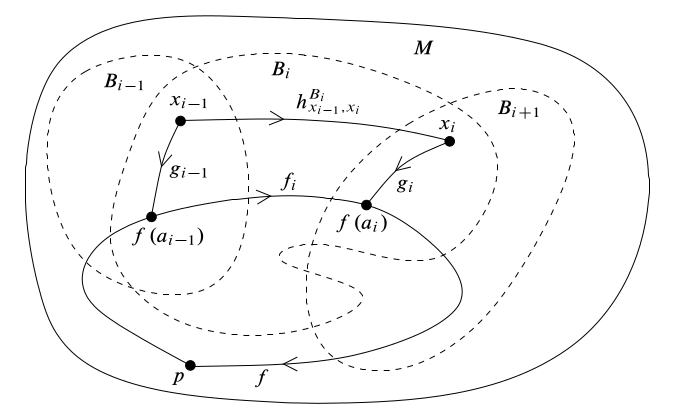
\includegraphics[width=0.5\textwidth]{manifold-fundamental-group.png}
        \label{fig:manifold-fundamental-group-png}
    \end{figure}

    \subsection*{Smooth Structures}
            We have the foundations to study topological properties of topological
            manifolds, however, we want to introduce certain properties from calculus such
            as derivatives to manifolds.\\
            However, derivatives in the typical sense don't make sense since they are not
            invariant under homeomorphisms. For example, the map $\varphi  \colon
            \mathbb{R}^2 \to \mathbb{R}^2$ given by $\varphi \left( u,v \right) 
            = \left( u^{\frac{1}{3}}, v^{\frac{1}{3}} \right) $ is a homeomorphism, but
            while
            $f  \colon \mathbb{R}^2 \to \mathbb{R}$ given by $f(x,y) = x$ is differentiable
            everywhere, the map $f \circ \varphi$ is not differentiable at the origin.\\
            \linebreak
            To make sense of derivatives of real-valued functions, curves, or maps between
            manifolds, we need to introduce a new kind of manifold called a \textit{smooth
            manifold}. It will be a topological manifold with some extra structure in
            addition to its topology.\\
            \linebreak
            The definition will be based on the calculus of maps between Euclidean spaces,
            so let us begin by reviewing some basic terminology about such maps.
            \begin{definition}[Smooth maps]
                If $U$ and $V$ are open subsets of $\mathbb{R}^{n}$ and $\mathbb{R}^{m}$,
                respectively, a function $F  \colon U \to V$ is said to be
                \textbf{smooth} (or \textbf{$C^{\infty}$}, or \textbf{infinitely
                differentiable}) if each of its component functions has continuous partial
                derivatives of all orders.
            \end{definition}
            \begin{definition}[Diffeomorphism]
                If a smooth map $F  \colon U \to V$ is bijetive and has a smooth inverse
                map, it is called a \textbf{diffeomorphism}.
            \end{definition}
            To see what additional structure on a topological manifold might be appropriate
            for discerning which maps are smooth, consider an arbitrary topological
            $n$-manifold $M$. Each point in $M$ is in the domain of a coordinate map
            $\varphi  \colon U \to \hat{U}\subset \mathbb{R}^{n}$.\\
            A plausible definition of a smooth function on $M$ would be to say that
            $f  \colon M \to \mathbb{R}$ is smooth if and only if the composite function
            $f \circ \varphi^{-1}  \colon \hat{U} \to \mathbb{R}$ is smooth in the sense of
            ordinary calculus. But this will make sense only if this property is
            independent of the choice of coordinate chart. Since smoothness is not
            a homeomorphism-invariant property, we consider the collection of all smooth
            charts as a new kind of structure on $M$.\\
            \linebreak
            With this in mind, we describe the construction:

            \begin{definition}[Transition maps]
                Let now $M$ be a topological $n$-manifold. If $\left( U, \varphi \right) $ 
            and $(V, \psi)$ are two charts such that $U \cap V \neq \varnothing$, the
            composite map $\psi \circ \varphi^{-1}  \colon
            \varphi \left( U \cap V \right) \to \psi \left( U \cap V \right) $ is called 
            the \textbf{transition map from $\varphi$ to $\psi$}.
            \end{definition}
            It is a composition of homeomorphisms and therefore a homeomorphism.
            \begin{definition}[Smoothly compatible]
                Two charts $\left( U, \varphi \right) $ and $\left( V, \psi \right) $ are
                said to be \textbf{smoothly compatible} if either $U \cap V = \varnothing$ 
                or the transition map $\psi \circ \varphi^{-1}$ is a diffeomorphism.
            \end{definition}
            \begin{definition}[Atlas]
                An \textbf{atlas for $M$} is a collection of charts whose domains cover
                $M$. An atlas $\mathcal{A}$ is called a \textbf{smooth atlas} if any two
                charts in $\mathcal{A}$ are smoothly compatible with each other.
            \end{definition}
            To show that an atlas is smooth, we thus need to verify that each transition
            map $\psi \circ \varphi^{-1}$ is smooth whenever $\left( U, \varphi \right)
            $ and
            $\left( V, \psi \right) $ are charts in $\mathcal{A}$ ; then it follows that
            $\psi \circ \varphi^{-1}$ is a diffeomorphism because the transition map
            $\varphi \circ \psi^{-1}$ is clearly its inverse and also a transition map,
            hence smooth. Therefore $\psi \circ \varphi^{-1}$ is smooth and has a smooth
            inverse, and is bijective on $\varphi \left( U \cap V \right) 
            \to \psi \left( U \cap V \right) $ since it is a homeomorphism.\\

            \begin{remark}
                Alternatively, given two particular charts $\left( U, \varphi \right) $ and
                $\left( V, \psi \right) $, it is often easier to show that they are
                smoothly compatible by verifying that $\psi \circ \varphi^{-1}$ is smooth
                and injective with nonsingular Jacobian at each point which gives that
                $\psi \circ \varphi^{-1}$ is a diffeomorphism onto its image by Corollary
                \ref{corollary-inverse-function-thm}.
            \end{remark}

            Our plan now is to define a "smooth structure" on $M$ by defining a smooth
            atlas, and to define a function $f  \colon M \to \mathbb{R}$ to be smooth if
            and only if $f \circ \varphi^{-1}$ is smooth in the sense of ordinary calculus
            for each coordinate chart $\left( U, \varphi \right) $ in the atlas.
            There is one problem though: in general, there will be many possible atlases
            that give the "same" smooth structure, in that they all determine the same
            collection of smooth functions on $M$. For example, consider the following pair
            of atlases on $\mathbb{R}^{n}$ :
                \begin{align*}
                \mathcal{A}_1 &= \left\{ \left( \mathbb{R}^{n}, \id_{\mathbb{R}^{n}}
                \right)  \right\} \\
                        \mathcal{A}_2 &=
                        \left\{ \left( B_1 (x), \id_{B_1(x)} \right)  \colon
                        x \in  \mathbb{R}^{n} \right\}.
            \end{align*}
            Although these are different smooth atlases, a function
            $f  \colon \mathbb{R}^{n} \to \mathbb{R}$ is smooth with respect to either
            atlas if and only if it is smooth in the sense of ordinary calculus.\\
            \linebreak
            We could choose to define a smooth structure as an equivalence class of smooth
            atlases under an appropriate equivalence relation. However, it is more
            straightforward to make the following definition:

            \begin{definition}[Maximal smooth atlas]
            A smooth atlas $\mathcal{A}$ on $M$ is \textbf{maximal} if it is not
            properly contained in any larger smooth atlas.\\
            (Such a smooth atlas is also said to be \textbf{complete})
            \end{definition}
            Now we can define the main concept of this chapter.

            \begin{definition}[Smooth structure]
            If $M$ is a topological manifold, a \textbf{smooth structure on $M$} is
            a maximal smooth atlas.\\
            Smooth structures are also called \textbf{differentiable structures} or
            \textbf{$C^{\infty}$ structures} by some authors.
            \end{definition}

            \begin{definition}[Smooth manifold]
            A \textbf{smooth manifold} is a pair $\left( M, \mathcal{A} \right) $ where
            $M$ is a topological manifold and $\mathcal{A}$ is a smooth structure on
            $M$.\\
            We also use the term \textbf{smooth manifold structure} to mean a manifold
            topology together with a smooth structure.
            \end{definition}

            \begin{remark}
            It is not always possible to find a smooth structure on a given topological
            manifold: there exist topological manifolds that admit no smooth structure
            at all (the first example was a compact $10$-dimensional manifold found in
            1960 by Michel Kervaire).
            \end{remark}

            \begin{proposition}[]
            Let $M$ be a topological manifold.
            \begin{enumerate}
                \item Every smooth atlas $\mathcal{A}$ for $M$ is contained in a unique
                    maximal smooth atlas, called the
                    \textbf{smooth structure determined by $\mathcal{A}$}.
                \item Two smooth atlases for $M$ determine the same smooth structure if
                    and only if their union is a smooth atlas.
            \end{enumerate}
            \end{proposition}


            \begin{proof}
            \begin{figure}[H]
                \centering
                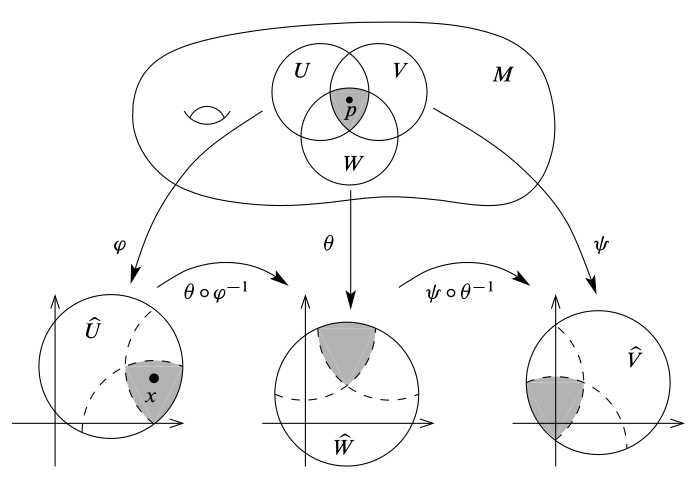
\includegraphics[width=0.6\textwidth]{prop-1-17-a.png}
                \label{fig:prop-1-17-a-png}
            \end{figure}
            (1): Let $\mathcal{C}$ be the collection of all
            smooth atlases containing $\mathcal{A}$, i.e.,
            $\forall C \in \mathcal{C} \colon \mathcal{A}\subset C$.\\
            We claim that $\mathcal{B}= \bigcup_{C \in \mathcal{C}} C$ is a smooth
            atlas. To show this, let
            $\left( U, \varphi \right) ,
            \left( V, \psi \right) \in 
            \mathcal{B}$. We must show that
            the two charts are smoothly compatible. Suppose
            $U \cap V \neq \varnothing$. Let
            $p \in U \cap V$. There
            exist smooth atlases $C,C' \in \mathcal{C}$ such that
            $\left( U, \varphi \right) \in C$ and
            $\left( V, \psi \right) \in C'$. Each of these contain
            $\mathcal{A}$ by definition, and since $\mathcal{A}$ is a smooth atlas,
            there exists some chart $\left( W, \theta \right) 
            \in \mathcal{A}$ such that $p \in W$. By $C$ being a smooth atlas
            and  $p \in U \cap W$, the map
            $\varphi \circ \theta^{-1}$ is a diffeomorphism, and
            since $C'$ is smooth too, the map
            $\theta \circ \psi^{-1}$ is a diffeomorphism. Thus the composition
            $\varphi \circ \psi^{-1} =
            \varphi \circ \theta^{-1} \circ \theta \circ \psi^{-1}$ is
            a diffeomorphism. Similarly, $\psi \circ \varphi^{-1}$ is a diffeomorphism.
            Thus $\mathcal{B}$ is a smooth atlas.\\
            To check maximality, suppose $\mathcal{B}'$ is a smooth atlas containing
            $\mathcal{B}$. Then $\mathcal{B'}$ in particular contains
            $\mathcal{A}$, so $\mathcal{B}' \in \mathcal{C}$, so
            $\mathcal{B'} \subset \mathcal{B}$. Hence
            $\mathcal{B} = \mathcal{B'}$.\\
            Suppose now $\mathcal{B}'$ is another maximal smooth atlas containing
            $\mathcal{A}$. Then in particular $\mathcal{B}'
            \in \mathcal{C}$, so $\mathcal{B}' \subset \mathcal{B}$, and by
            maximality of $\mathcal{B}'$, we have $\mathcal{B}' = \mathcal{B}$.\\
            \linebreak
            (2): Suppose $\mathcal{A}, \mathcal{A}'$ are smooth structures that
            determine the same smooth structure on $M$, say $\mathcal{B}$. Then
            $\mathcal{A}, \mathcal{A}' \subset \mathcal{B}$, so
            in particular, any chart of $\mathcal{A}$ is smoothly compatible with any
            chart of $\mathcal{A}'$, so 
            $\mathcal{A} \cup \mathcal{A}'$ is a smooth atlas.\\
            Conversely, if $\mathcal{A}\cup \mathcal{A}'$ is a smooth atlas, then
            by (a), $\mathcal{A}$ is contained in a unique maximal smooth atlas, call
            it $\mathcal{B}$, and similarly, $\mathcal{A}'$ is contained in a unique
            maximal smooth atlas, call it $\mathcal{B}'$, both of which was the set of
            charts which are smoothly compatible with every chart in
            $\mathcal{A}$ and $\mathcal{A}'$, respectively. I.e., 
            $\mathcal{A} \cup \mathcal{A}' \subset \mathcal{B},\mathcal{B}'$, so
            by uniqueness, $\mathcal{B} = \mathcal{B}'$.
            \end{proof}


            \begin{example}[]
            If a topological manifold $M$ can be covered by a single chart, the smooth
            compatibility condition is trivially satisfied, so any such chart
            automatically determines a smooth structure on $M$.\\
            \end{example}

            \begin{remark}
            If we replace the requirement that the carts be smoothly compatible by
            the weaker requirement that each transition map
            $\psi \circ \varphi^{-1}$ (and its inverse) be of class
            $C^{k}$, we obtain the definition of a \textbf{$C^{k}$ structure}.
            Similarly, if we require that each transition map be real-analytic
            (expressible as a convergent power series in a neighborhood of each point),
            we obtain the definition of a \textbf{real-analytic} structure, also called
            a $C^{\omega }$ structure. If $M$ has even dimension $n=2m$, we can
            identify $\mathbb{R}^{2m}$ with $\mathbb{C}^{m}$ and require that the
            transition maps be complex-analytic; this determines a 
            \textbf{complex-analytic structure}. A manifold endowed with one of these
            structures is called a \textbf{$C^{k}$ manifold, real-analytic manifold},
            or \textbf{complex manifold}, respectively. (Note that a
            $C^{0}$ manifold is just a topological manifold).
            \end{remark}


    \subsection*{Local Coordinate Representations}
        \begin{definition}[]
        If $M$ is a smooth manifold, any chart $\left( U, \varphi \right)
        $ contained in the given maximal smooth atlas is called a \textbf{smooth
        chart}, and the corresponding coordinate map $\varphi$ is called
        a \textbf{smooth coordinate map}. It is useful also to introduce the terms
        \textbf{smooth coordinate domain} or \textbf{smooth coordinate
        neighborhood} for the domain of a smooth coordinate chart. 
        A \textbf{smooth coordinate ball} means a smooth coordinate domain whose
        image under a smooth coordinate map is a ball in Euclidean space. 
        A \textbf{smooth coordinate cube} is defined similarly.
        \end{definition}

        \begin{definition}[Regular coordinate ball]
        A set $B \subset M$ is a \textbf{regular coordinate ball} if there is
        a smooth coordinate ball $B' \supset \overline{B}$ and a smooth coordinate
        map $\varphi  \colon B' \to \mathbb{R}^{n}$ such that for some positive
        real numbers $r < r'$,
        \[
        \varphi (B) = B_r (0), \quad \varphi \left( \overline{B} \right) 
        = \overline{B}_r (0), \quad \text{and} \quad
        \varphi \left( B' \right) = B_{r'}(0).
        \] 
        \end{definition}
        Because $\overline{B}$ is homeomorphic to $\overline{B}_r (0)$, it is compact,
        and thus every regular coordinate ball is precompact in $M$.

        \begin{proposition}[]\label{regular-coordinate-ball-basis}
        Every smooth manifold has a countable basis of regular coordinate balls.
        \end{proposition}

        \begin{proof}
        Let $M$ be a smooth manifold of dimension $n$. Suppose first that
        $M$ can be covered by one chart $\left( U, \varphi \right) $. 
        The balls at rational coordinates of $\mathbb{R}^{n}$ with rational
        radii are a basis for the topology of $\varphi(U)$ and also
        $\mathbb{R}^{n}$, so in particular, the preimage of these balls under
        $\varphi$ is a basis for the topology on $M$.\\
        Suppose now that we have a collection of charts
        $\left\{ U_{\alpha}, \varphi_{\alpha} \right\} $ covering $M$.
        By the single chart case, each of these charts has a countable basis of
        regular coordinate balls, and since $\bigcup_{\alpha} U_{\alpha}$ covers
        covers $M$, and thus there is a countable union of countable bases, which
        is countable and a basis for $M$.\\
        We must also argue that the closure of a regular coordinate ball in
        $U_{\alpha}$ is the same as its closure in $M$. Its closure is compact in
        $U_{\alpha}$ as the image under $\varphi$ of its closure is compact and
        $\varphi$ is a homeomorphism. So it is compact in $M$ too and since $M$ is Hausdorff,
        the closure  in $U_{\alpha}$ is closed in $M$ too, hence the closures are
        the same.
        \end{proof}

        \begin{note}
         We can represent a point $p \in M$ by its coordinates
         in a chart $\left( U, \varphi \right) $: 
         $\left( x^{1}, \ldots, x^{n} \right) = \varphi(p)$, and think of this
         $n$-tuple as \textit{being} the point $p$. We typically express this by
         saying "$\left( x^{1}, \ldots, x^{n} \right) $ is the (local) coordinate
         representation for $p$ " or "$p = \left( x^{1},\ldots,
         x^{n}\right) $ in local coordinates".\\
         Another way to look at it is that by means of our identification
         $U \leftrightarrow \hat{U}$, we can think of $\varphi$ as the identity map
         and suppress it from notation. One needs to remember that the
         identification is in general only local, and depends heavily on the choice
         of coordinate chart.
        \end{note}

    \subsection*{Examples of Smooth Manifolds}
        \begin{example}[0-Dimensional Manifolds]
         A topological manifold $M$ of dimension $0$ is just a countable discrete
         space. For each point $p \in M$, the only neighborhood of $p$ that is
         homeomorphic to an open subset of $\mathbb{R}^{0}$ is 
         $\left\{ p \right\} $ itself, and there is exactly one coordinate map
         $\varphi  \colon \left\{ p \right\} \to \mathbb{R}^{0}$. Thus, the set of
         all charts on $M$ trivially satisfies the smooth compatibility condition,
         and each $0$-dimensional manifold has a unique smooth structure.
        \end{example}

        \begin{example}[Euclidean Spaces]
         For each nonnegative integer $n$, the Euclidean space
         $\mathbb{R}^{n}$ is a smooth $n$-manifold with the smooth structure
         determined by the atlas consisting of the single chart $\left(
         \mathbb{R}^{n}, \id_{\mathbb{R}^{n}} \right) $. We call this the
         \textbf{standard smooth structure on $\mathbb{R}^{n}$} and the resulting
         coordinate map \textbf{standard coordinates}. Unless we explicitly specify
         otherwise, we always use this smooth structure on $\mathbb{R}^{n}$. With
         respect to this smooth structure, the smooth coordinate charts for
         $\mathbb{R}^{n}$ are exactly those charts $\left( U, \varphi \right)
         $ such that $\varphi$ is a diffeomorphism (in the sense of ordinary
         calculus) from $U$ to another open subset $\hat{U} \subset
         \mathbb{R}^{n}$.
        \end{example}

        \begin{example}[A different smooth structure on $\mathbb{R}$]
         Consider the homeomorphism $\psi  \colon \mathbb{R} \to \mathbb{R}$ given
         by
         \[
         \psi(x) = x^3.
         \] 
         The atlas consisting of the single chart $\left( \mathbb{R}, \psi \right)
         $ defines a smooth structure on $\mathbb{R}$ that is different from the
         standard smooth structure because the transition map
         $\id_{\mathbb{R}} \circ \psi^{-1} (y) = y^{\frac{1}{3}}$ is not smooth at
         the origin. Using similar ideas, it is not hard to construct many distinct
         smooth structures on any given positive-dimensional topological manifold,
         as long as it has one smooth structure to begin with.
        \end{example}

        \begin{example}[Finite-Dimensional Vector Spaces]
         Let $V$ be a finite-dimensional real vector space. Any norm on $V$ 
         determines a topology, which is independent of the choice of norm. With
         this topology, $V$ is a topological $n$-manifold, and has a natural smooth
         structure defiend as follows. Each ordered basis
         $\left( e_1, \ldots, e_n \right) $ for $V$ defines a basis isomorphism
         $e  \colon \mathbb{R}^{n} \to V$ by
         \[
         e(x) = \sum_{i=1}^{n} x^{i} e_i.
         \] 
         This map is a homeomorphism, so $\left( V, e^{-1} \right) $ is a chart. If
         $\left( \tilde{e_1}, \ldots,
         \tilde{e_n} \right) $ is any other basis and
         $\tilde{e}(x) = \sum_{j} x^{j}\tilde{e_j} $ i the corresponding
         isomorphism, then there is some invertible matrix
         $\left( A_{i}^{j} \right) $ such that
         $e_i = \sum_j A_{i}^{j} \tilde{e_j}$ for each $i$. The transition map
         between the two charts is then given by
         $\tilde{e}^{-1} \circ e(x) = \tilde{x}$, where $\tilde{x}
         = \left( \tilde{x}^{1},\ldots, \tilde{x}^{n} \right) $
         is determined by
         \[
         \sum_{j=1}^{n} \tilde{x}^{j} \tilde{E}_j =
         \sum_{i=1}^{n} x^{i} E_i = \sum_{i,j=1}^{n} x^{i}A_{i}^{j}\tilde{E}_j.
         \] 
         It follows that $\tilde{x}^{j}=
         \sum_i A_i^{j} x^{i}$. Thus, the map sending $x$ to $\tilde{x}$ is an
         invertible linear map and hence a diffeomorphism, so any two such charts
         are smoothly compatible. The collection of all such charts thus defines
         a smooth structure, called the \textbf{standard smooth structure on $V$}.     
        \end{example}

        \begin{example}[Open submanifolds]
            Let $M$ be a smooth $n$-manifold and let $U \subset M$ be any open subset.
            Define an atlas on $U$ by
            \[
            \mathcal{A}_{U} = \left\{ \text{smooth charts }
            \left( V,\varphi \right) \text{ for }M \text{ such that }
            V \subset U \right\} .
            \] 
            Every point $p \in U$ is contained in the domain of some chart
            $\left( W, \varphi \right) $ for $M$ ; if we set
            $V = W \cap U$, then $\left( V, \varphi|_{V} \right) $ is a chart in
            $\mathcal{A}_U$ whose domain contains $p$. Therefore $U$ is covered by the
            domains of charts in $\mathcal{A}_U$, and it is easy to verify that this is
            a smooth atlas for $U$. Thus any open subset of $M$ is itself a smooth
            $n$-manifold in a natural way. Endowed with this smooth structure, we call
            any open subset an \textbf{open submanifold of $M$}. (We will define a more
            general class of submanifolds in chapter 5)
        \end{example}
        
        \begin{example}[Spheres]
            The $n$-sphere $S^{n}\subset \mathbb{R}^{n+1}$ is a topological
            $n$-manifold. We put a smooth structure on $S^{n}$ as follows.
            For each $i = 1, \ldots, n+1$, let
            $\left( U_i^{\pm}, \varphi_i^{\pm} \right) $ denote the graph
            coordinate charts 
            $\varphi_i^{\pm}  \colon U_i^{\pm} \cap S^{n} \to B^{n}$ given by
            \[
            \varphi_i^{\pm} \left( x^{1},\ldots, x^{n+1} \right) 
            = \left( x^{1}, \ldots, \hat{x^{i}},
            \ldots, x^{n+1}\right) ,
            \] 
            where $U_i^{+} =
            \left\{ \left( x^{1},\ldots, x^{n+1} \right) \in \mathbb{R}^{n+1} \colon
            x^{i}>0\right\} $ and $U_i^{-}$ is defined similarly with
            $x^{i}<0$.\\
            For any indices $i$ and $j$, the transition map
            $\varphi_i^{\pm} \circ \left( \varphi_j^{\pm} \right)^{-1}$ is
            easily computed. In the case $i<j$, we get
            \[
            \varphi_i^{\pm}\circ \left( \varphi_j^{\pm} \right)^{-1}
            \left( u_1, \ldots, u_{n} \right) 
            = \left( u_1, \ldots, \hat{u_i},\ldots,
            \pm \sqrt{1- \left| u \right|^2} ,\ldots,
            u^{n}\right) 
            \] 
            with the square root in the $j$ th position. A similar formula
            holds for $i>j$. When $i = j$, we get
            $\varphi_i^{+} \circ \left( \varphi_i^{+} \right)^{-1}
            = \varphi_i^{-} \circ \left( \varphi_i^{-} \right)^{-1}
            = \id_{B^{n}}$. Thus, the collection of charts
            $\left\{ \left( U_i^{\pm}, \varphi_i^{\pm} \right)  \right\} $ is
            a smooth atlas, and so defines a smooth structure on $S^{n}$. We
            call this its \textbf{standard smooth structure}.
        \end{example}

        \begin{example}[Level sets]
            We can generalize the preceding example as follows. 
            Suppose $U \subset \mathbb{R}^{n}$ is an open subset and
            $\Phi  \colon U \to \mathbb{R}$ is a smooth function.
            For any $c \in \mathbb{R}$, the set $\Phi^{-1}(c)$ is called a
            \textbf{level set of $\Phi$}. Choose some $c \in \mathbb{R}$, let
            $M = \Phi^{-1}(c)$, and suppose it happens that the total
            derivative $D \Phi(a)$ is nonzero for each  $a \in \Phi^{-1}(c)$.
            Because $D \Phi(a)$ is a row matrix whose entries are the partial
            derivatives  $\left( \frac{\partial \Phi}{\partial x^{1}}(a),
            \ldots, \frac{\partial \Phi}{\partial x^{n}} (a) \right)$, for each
            $a$ there is some $i$ such that 
            $\frac{\partial \Phi}{\partial x^{i}} (a) \neq 0$.\\
            It follows from the implicit function theorem
            (Theorem \ref{implicit-function-thm}) that there is
            a neighborhood $U_0$ of $a$ such that $M \cap U_0$ can be expressed
            as a graph of  an equation of the form
            \[
            x^{i} = f\left( x^{1},\ldots, \hat{x^{i}},\ldots
            ,x^{n} \right),
            \] 
            for some smooth real-valued $f$ defined on an open subset of
            $\mathbb{R}^{n-1}$. Therefore, arguing just as in the case of the
            $n$-sphere, we see that $M$ is a topological manifold of dimension 
            $(n-1)$, and has a smooth structure such that each of the graph
            coordinate charts associated with a choice of $f$ as above is
            a smooth chart. 
        \end{example}

        \begin{example}[Projective Spaces]
            The $n$-dimensional real projective space
            $\mathbb{R}\mathbb{P}^{n}$ is a topological $n$-manifold. Let us
            check that the coordinate charts 
            $\varphi_i  \colon U_i \to \mathbb{R}^{n}$, where
            $U_i = \pi \left( \tilde{U_i} \right) $ with
            $\tilde{U_i} \subset \mathbb{R}^{n+1}-\left\{ = \right\} $ is the
            set where $x^{i} \neq 0$, and
            \[
            \varphi_i \left[ x^{1},\ldots, x^{n+1} \right] 
            = \left( \frac{x^{1}}{x^{i}},\ldots,
            \frac{x^{i-1}}{x^{i}}, \frac{x^{i+1}}{x^{i}}, \ldots,
            \frac{x^{n+1}}{x^{i}}
        \right) 
            \] 
            are smoothly compatible. Assume $i > j$. THen
            \[
            \varphi_j \circ \varphi_i^{-1} \left( u^{1},\ldots, u^{n}\right) 
            =
            \left( \frac{u^{1}}{u^{j}},\ldots,
                \frac{u^{j-1}}{u^{j}}, \frac{u^{j+1}}{u^{j}},\ldots,
                \ldots,
                \frac{u^{i-1}}{u^{j}}, \frac{1}{u^{j}},
                \frac{u^{i}}{u^{j}},\ldots,
                \frac{u^{n}}{u^{j}}
            \right) 
            \] 
            which is a diffeomorphism from
            $\varphi_i\left( U_i \cap U_j \right) $ to
            $\varphi_j \left( U_i \cap U_j \right) $.
        \end{example}

        \begin{example}[Smooth Product Manifold]
            If $M_1, \ldots, M_k$ are smooth manifolds of dimension
            $n_1, \ldots, n_k$, $M_1 \times \ldots \times M_k$ is a topological
            manifold of dimension $n_1 + \ldots + n_k$, with charts of the form
            $\left( U_1 \times \ldots \times U_k, 
            \varphi_1 \times \ldots \times \varphi_k \right) $. Any two charts
            are smoothly compatible because
            \[
                \left( \psi_1 \times \ldots \times \psi_k \right) \circ
                \left( \varphi_1 \times \ldots \times \varphi_k \right)^{-1}
                =
                \left( \psi_1 \circ \varphi_1^{-1} \right) \times \ldots
                \times  \left( \psi_k \circ \varphi_k^{-1} \right) 
            \] 
            is a smooth map. This defines a natural smooth manifold structure
            on the product, called the \textbf{product smooth manifold
            structure}.\\
            For example, this yields a smooth manifold structure on the
            $n$-torus $T^{n} = S^{1} \times \ldots \times S^{1}$.
        \end{example}


        \begin{lemma}[Smooth Manifold Chart Lemma]
            Let $M$ be a set, and suppose we are given a collection
            $\left\{ U_{\alpha} \right\} $ of subsets of
            $M$ together with maps $\varphi_{\alpha}  \colon
            U_{\alpha}  \to \mathbb{R}^{n}$, such that the following properties
            are satisfied:
            \begin{enumerate}
                \item For each $\alpha, \varphi_{\alpha}$ is a bijection
                    between $U_{\alpha}$ and an open subset
                    $\varphi_{\alpha}\left( U_{\alpha} \right) \subset 
                    \mathbb{R}^{n}$.
                \item For each $\alpha$ and $\beta$, the sets
                    $\varphi_{\alpha}\left( U_{\alpha}\cap U_{\beta} \right) $ 
                    and $\varphi_{\beta}\left( U_{\alpha} \cap U_{\beta}
                    \right) $ are open in $\mathbb{R}^{n}$.
                \item Whenever $U_{\alpha} \cap U_{\beta} \neq \varnothing$,
                    the map $\varphi_{\beta} \circ \varphi_{\alpha}^{-1}  \colon
                    \varphi_{\alpha} \left( U_{\alpha}\cap U_{\beta} \right) \to 
                    \varphi_{\beta} \left( U_{\alpha}\cap U_{\beta} \right)
                    $ is smooth.
                \item Countably many of the sets $U_{\alpha}$ cover $M$.
                \item Whenever $p,q$ are distinct points in $M$, either there
                    exists some $U_{\alpha}$ containing both $p$ and $q$ or
                    there exist disjoint sets $U_{\alpha},U_{\beta}$ with
                    $p \in U_{\alpha}$ and $q \in U_{\beta}$.
            \end{enumerate}
            Then $M$ has a unique smooth manifold structure such that each
            $\left( U_{\alpha}, \varphi_{\alpha} \right) $ is a smooth chart.
        \end{lemma}

        \begin{example}[Grassmannian]
            Checking Hausdorff condition: Suppose
            $P, P' \subset V$ are $k$-dimensional subspaces and $V$ is
            an $n$-dimensional space. 
        \end{example}

        \begin{exercise}[]
            Show that every smooth manifold with boundary has a 
            countable basis
            consisiting of regular coordinate balls and half-balls.
        \end{exercise}

        \begin{solution}
            Suppose first $M$ is covered by some chart
            $\left( U, \varphi \right) $. If
            $\varphi$ maps into $\mathbb{R}^{n}$, then
            $\partial M = \varnothing$, and we are done.
            Hence suppose $\varphi  \colon
            U \to \mathbb{H}^{n}$, and
            $\varphi(x) = 0$ without loss of generality.
            Then since $U$ is open, there exist some
            $r' > r > 0$ such that
            \[
                \overline{B}_r(0) \cap \mathbb{H}^{n}
                \subset 
                B_{r'}(0) \cap \mathbb{H}^{n}
                \subset \varphi(U).
            \] 
            Let
            $B = \varphi^{-1}\left( 
            B_r(0) \cap \mathbb{H}^{n} \right) $ and
            $B' = \varphi^{-1}\left( 
            B_{r'}(0) \cap \mathbb{H}^{n}\right) $.
            Since $\varphi$ is a homeomorphism, we have
            $\overline{B} =
            \overline{\varphi^{-1}\left( 
            B_r(0) \cap \mathbb{H}^{n}\right) }
            = \varphi^{-1}\left( 
            \overline{B_r(0) \cap \mathbb{H}^{n}}\right) $, hence
            $\varphi\left( \overline{B} \right) 
            = \overline{B}_r(0) \cap \mathbb{H}^{n}$.
            Thus $B$ is a regular coordinate half-ball
            at $x$ contained in $U$.\\
            Let
            $\mathcal{B}$ be the collection of all preimages
            $\varphi^{-1}\left( 
            B_s(t) \right) $ and
            $\varphi^{-1}\left( B_s(t) \cap \mathbb{H}^{n} \right) $
            with $s \in \mathbb{Q}$ and
            $t \in \mathbb{Q}^{n}$. Then
            $\mathcal{B}$ is a countable basis for $M$.\\
            Now suppose $M$ is an arbitrary $n$-manifold with
            boundary. Then there is a countable collection
            of charts that cover $M$ and each domain has by the above
            a countable collection of regular coordinate balls and 
            half-balls as a basis, and since each domain is open, these
            are also open in $M$. Further, suppose
            $B$ is a regular coordinate ball in some domain of a chart
            $U_{\alpha}$. We must also argue that the
            closure in $U_{\alpha}$ of $B$ is the same as
            its closure in $M$. Now, its closure in
            $U_{\alpha}$ is compact, and since $M$ is Hausdorff,
            compact subsets are closed, so the closure 
            of $B$ in $U_{\alpha}$ is also closed in $M$.
            Thus the closures coincide.
        \end{solution}

        \begin{remark}
            The idea for this problem is that each point in
            $M$ is contained in a chart $\left( U, \varphi \right) $.
            Since $U$ is a manifold with the induced topology, 
            we simply prove it for the case of $M$ being coverable
            with a single chart first. Then we have that
            the topology for $U$ as a subspace has a countable
            basis of regular coordinate balls and half-balls.
            Now since a countable collection of charts
            cover $M$ (by second-countability), we wish to
            conclude that the union of the collections of
            regular coordinate balls and half-balls for the individual
            chart domains is a countable basis of regular coordinate
            balls and half-balls. For this, we need to be careful
            that the topological properties carry over. 
            Openness carries over as each chart domain is open.
            And closures carry over since the closure is
            compact in $U$, and hence also in $M$ and since
            $M$ is Hausdorff, it is closed in $M$ as well. 
            Hence the closures coincide as well. We thus see
            that Heine-Borel for $\mathbb{R}^{n}$ is important
            for us here.
        \end{remark}

    \subsection*{Problems}

    \begin{problem}
        Let $X$ be the set of all points
        $(x,y) \in \mathbb{R}^2$ such that
        $y = \pm 1$, and let $M$ be the quotient of
        $X$ by the equivalence relation generated
        by $\left( x,-1 \right) \sim \left( x,1 \right) $ 
        for all $x\neq 0$. Show that $M$ is locally Euclidean
        and second-countable, but not Hausdorff.
        (This space is called the \textbf{line with two
        origins})
    \end{problem}


    \begin{proof}
        Let $\pi  \colon X \to M$ be the quotient map.
        We first show that $\pi$ is open.
        Let $U \subset X$ be open. Then
        $\pi(U)$ is open iff $\pi^{-1}\left( p
        \left( U \right) \right) $ is open. Define
        $\varphi  \colon X \to X$ by
        $\varphi(x,y) = (x,-y)$. Then
         \[
        \pi^{-1}\left( p(U) \right) 
        = U \cup \varphi \left( U - \left\{ 
        (0,1) , (0,-1) \right\}  \right) 
        \] 
        which is open as $\varphi$ is a homeomorphism. 
        Hence $\pi$ is an open map.\\
        We can define a map $f  \colon
        M \to \mathbb{R}$ by
        $f (\overline{x}) = \pi_1 \left( \pi^{-1}(x) \right) $ where
        $\pi_1$ here is the projection onto the first coordinate (this
        is the induced map in the diagram below).
        So for $\pi (x,1) \in M$, we have
        $f\left( \pi (x,1) \right) = x$.
        We claim that $f$ also is an open map. Firstly, since
        $f \circ \pi  \colon X \to \mathbb{R}$ is simply the projection
        onto the first coordinate and $\pi$ is a quotient map,
        we have that $f$ is continuous. Now, further, since
        projections are open and since $\pi$ is open, we must have
        that $f$ is open too.
        \begin{equation*}
        \begin{tikzcd}
            X \ar[rr, "\pi_1"] \ar[ddr, "\pi"] && \mathbb{R}\\
                                     &&\\
                                     &M \ar[uur, "f", dashed]&
        \end{tikzcd}
        \end{equation*}
        Now we show that $M$ is locally Euclidean.\\
        Suppose $\overline{x}\in M$. Then we can assume without loss of
        generality that  $\overline{x}= \pi \left( x,1 \right) $ 
        ($\pi\left( x,-1 \right) $ is similar).
        Then $\pi_1 \left( \left( x-\varepsilon, x+\varepsilon \right) 
        \times  \left\{ 1 \right\} \right) $ is an open set
        around $f\left( \overline{x} \right) $.\\
        To show that it is second-countable, 
        note that since $\pi$ is a quotient map, the preimage of any
        open subset of $M$ is open in $X$, but the topology
        of $X$ has basis of all balls in
        $\mathbb{R}^2$ with rational coordinates and rational radii, so
        the images of these under $\pi$ which is open are also open
        and hence form a basis for $M$.\\
        To see that $M$ is not Hausdorff, it is trivial to check that
        $\left( 0,1 \right) $ and $(0,-1)$ do not have
        disjoint neighborhoods.
    \end{proof}

    \begin{exercise}[]
        A topological space is said to be \textbf{$\sigma$-compact} if
        it can be expressed as a union of countably many compact
        subspaces. Show that a locally Euclidean Hausdorff space
        is a topological manifold if and only if it is
        $\sigma $-compact.
    \end{exercise}

    \begin{proof}
        Suppose $M$ is a locally Euclidean Hausdorff space. If
         we can show that any open subset of $M$ is contained in
         a compact subset, then second-countability together
         with $M$ being locally Euclidean would imply
         $\sigma $-compactness.\\
         Since any manifold has a countable basis of precompact
         coordinate balls, we can let $\mathcal{B}$ be such a basis.
         Then $\overline{\mathcal{B}}=
         \left\{ \overline{B}  \mid B \in \mathcal{B} \right\} $ is
         a countable collection of compact balls which cover
         $M$.\\
         Conversely, suppose $M$ is $\sigma $-compact. Let
         $\mathcal{A} = \left\{ A_{\alpha}  \colon
         \alpha \in J \right\} $ be a countable collection of compact
         subspaces covering $M$. 
         Let $x \in M$ and $U_x$ be a neighborhood of $x$ which
         by local Euclidean is homeomorphic by $\varphi_x$ to an
         open subset $\varphi_x \left( U_x \right) \subset
         \mathbb{R}^{n}$.
         Then the preimage under $\varphi_x$ of all balls
         with rational coordinates and rational radii is a basis for
         the induced topology of $U_x$ - which are also open in $M$ -;
         let us denote this collection of coordinate balls by
         $\mathcal{B}_x$.
         Now, suppose $A_{\alpha} \in \mathcal{A}$. Then
         $\bigcup_{x \in A_{\alpha}} U_x$ covers
         $A_{\alpha}$ and since $A_{\alpha}$ is compact, there exists
         a finite subcollection $U_{x_1}, \ldots, U_{x_n}$.
         Now suppose $V \subset M$ is open and $x \in V$. Then there
         exists $A_{\alpha} \in \mathcal{A}$ such that
         $x \in A_{\alpha}$. Hence there exists
          $i$ such that $x \in U_{x_i}$. Since $V \cap U_{x_i}$ is
          an open subset of $U_{x_i}$, there exists a coordinate ball
          $B$ such that $x \in B \subset V \cap U_{x_i}$.\\
          Thus we see that if
          $\mathcal{B}_{\alpha} =
          \bigcup_{i=1}^{n} \mathcal{B}_{x_i}$, then
          $\bigcup_{\alpha \in J} \bigcup_{B
          \in \mathcal{B}_{\alpha}} B$ is a basis for
          $M$ which is countable.
    \end{proof}


    \begin{exercise}[]
        Suppose $M$ is a locally Euclidean Hausdorff space.
        Show that $M$ is second-countable if and only if it is
        paracompact and has countably many connected components.
        \todo{Unsolved}
    \end{exercise}

    \begin{proof}
        $\left( \implies \right) $ : is clear.\\
        $\left( \impliedby \right) $: Assume $M$ only has one
        component.\\
        Since every topological manifold has an open cover of precompact
        coordinate balls and half-balls and $M$ is paracompact, the cover
        admits
        an open, locally finite refinement, call it $\mathcal{B}$. Thus, every
        element $U \in \mathcal{B}$ is open and contained in some
        precompact coordinate ball or half-ball.\\
        Let $x \in M$. Then $x$ has an open neighborhood $U_x$ such that
        $U_x$ intersects finitely many elements of $\mathcal{B}$. The
        collection $\bigcup_{x \in M} U_x$ covers $M$.
        
        \newpage
        Since $M$ is locally Euclidean, there exists a
        neighborhood $U_x$ for any $x \in M$ such that
        $\varphi_{x}  \colon U_x \to \hat{U}_x \subset \mathbb{R}^{n}$
        is a homeomorphism where $\hat{U}_x$ is open. Then
        the preimage of all regular 
        coordinate balls with rational coordinate
        and rational radius which is contained in $\hat{U}_x$ is
        a basis for the induced topology on $U_x$, denote this
        set by $\mathcal{B}_x$. That is, for each
        $B \in \mathcal{B}_x$, there exists $r' > r > 0$ such that
        $\varphi (\overline{B}) =
        \overline{B_r (y)} \subset B_{r'}(y) \subset \hat{U}_x$.\\
        Now, since
        $\bigcup_{x \in M} \bigcup_{B \in \mathcal{B}_x} B$ 
        covers $M$, there exists a locally finite open refinement,
        call it $\mathcal{B}$ which consists of precompact coordinate
        domains.\\
    \end{proof}

    \begin{exercise}[Complex projective $n$-space]
        Let $U \subset \mathbb{C}^{n+1} - \left\{ 0 \right\} $ 
        be open. Then
        $\pi^{-1} \left( \pi (U) \right) 
        = p^{-1} \left( p (U) \right) $ where
        $p  \colon \mathbb{C}^{n+1} - \left\{ 0 \right\} 
        \to S^{n}$ is the map
        $x \mapsto \frac{x}{\|x\|}$.
        Since if $\pi (x) \in \pi (U)$ then
        there exists $y \in U$ such that for some
        $\lambda \in \mathbb{R}_+$  we have
        $x = \lambda y$ and hence
        $\frac{x}{\|x\|} = \frac{\lambda y}{\|\lambda y\|}
        = \frac{y}{\|y\|}$, so 
        $p(x) = p(y) \in p\left( U \right) $. Conversely,
        if $p(x) \in p(U)$ then 
        $\frac{y}{\|y\|} = \frac{x}{\|x\|}$ for some $y \in U$, so
        $x = y \frac{\|x\|}{\|y\|}$ giving
        $\pi(x) = \pi(y)$.\\
        Since $p$ is continuous, $\pi$ is open. Since 
        $S^{n} \approx \mathbb{C}^{n+1} - \left\{ 0 \right\} $ and
        $p$ is also open, we further have that since
        $S^{n}$ is compact, so is $\mathbb{C}\mathbb{P}^{n}$.
    \end{exercise}

    \begin{proposition}[2.15 (Properties of Diffeomorphisms)]
        \begin{itemize}
            \item The restriction of a diffeo to an open 
                submanifold with or without boundary is a 
                diffeo onto its image.
            \item "Diffeomorphic" is an equivalence relation
                on the class of all smooth manifolds with
                or without boundary.
        \end{itemize}
    \end{proposition}

    \begin{proof}
        Suppose $F  \colon M \to N$ is a diffeomorphism, and
        let $U \subset M$ be an open subset inheriting
        the structure from $M$. Let
        $F(U)$ inherit the structure from $N$.
        Then for any $p \in U$, there exists a
        chart $\left( W, \varphi \right) $ around $p$ 
        in $M$ and $\left( V, \psi \right) $ around $F(p)$ in
        $N$ such that $\psi \circ F \circ \varphi^{-1}$ is
        diffeomorphic. Since $\psi|_{V \cap V} \circ F|_{U} \circ
        \left( \varphi|_{U \cap W} \right)^{-1} $ is also
        smooth, so  $F|_{U}$ is a diffeomorphism onto its
        image.\\
        \linebreak
        The second part is clear since the composition
        of diffeomorphisms is a diffeomorphism.
    \end{proof}
    



\newpage
\appendix
\section{Review of Calculus}
    \subsection*{Total and Partial Derivatives}
        \begin{definition}[Total derivative]
        Let $V$ and $W$ be finite-dimensional vector spaces, which we may assume to
        be endowed with norms. If $U \subset V$ is an open subset and
        $a \in U$, a map $F  \colon U \to W$ is said to be \textbf{differentiable
        at $a$} if there exists a linear map $L  \colon V \to W$ such that
        \begin{equation}
        \lim_{v \to 0} \frac{\left| F(a+v) - F(a) - Lv \right| }{\left| v \right|
        }=0 \label{eq:total-derivative}
        \end{equation}
        The norm in the numerator is that of $W$, while the norm in the denominator
        is that of $V$.\\
        If $F$ is differentiable at $a$, the linear map $L$ satisfying the above
        equation is denoted by $DF(a)$ and is called the \textbf{total derivative
        of $F$ at $a$}. Condition \eqref{eq:total-derivative} can also be written
        \[
        F(a+v) = F(a) + DF(a)v + R(v)
        \] 
        where the remainder term $R(v) = F(a+v) - F(a) - DF(a)v$ satisfies
        $\frac{\left| R(v) \right| }{\left| v \right| }\to 0$ as $v \to 0$. Thus
        the total derivative represents the "best linear approximation" to
        $F(a+v) - F(a)$ near $a$.
        \end{definition}

        \begin{proposition}[Chain Rule for Total
        Derivative]\label{chain-rule-total-derivative}
        Suppose $V,W,X$ are finite-dimensional vector spaces, $U \subset V$ and
        $\tilde{U}\subset W$ open subsets, and $F  \colon U \to \tilde{U}$ and
        $G  \colon \tilde{U} \to X$ maps. If $F$ is differentiable at
        $a \in U$ and $G$ is differentiable at $F(a) \in \tilde{U}$, then
        $G \circ F$ is differentiable at $a$, and
        \[
        D\left( G \circ F \right) (a) = DG\left( F(a) \right) \circ DF(a).
        \] 
        \end{proposition}

    \subsection*{Partial Derivatives}
        We now specialize to maps between Euclidean spaces.
        \begin{definition}[Jacobian]
            The matrix $\left( \frac{\partial F^{i}}{\partial x^{j}} \right) $ of
            partial derivatives is called the \textbf{Jacobian matrix of $F$}, and its
            determinant is called the \textbf{Jacobian determinant of $F$}.
        \end{definition}

        \begin{definition}[$C^{k}$ or $k$ times continuous differentiability]
        If $F  \colon U \to \mathbb{R}^{m}$ is a function for which each partial
        derivative exists at each point in $U$ and the functions
        $\frac{\partial F^{i}}{\partial x^{j}}  \colon U \to \mathbb{R}$ so defined
        are all continuous, then $F$ is said to be of
        \textbf{class $C^{1}$} or \textbf{continuously differentiable}.\\
        In general, if $U \subset \mathbb{R}^{n}$ is an open subset and $k \ge 0$,
        a function $F  \colon U \to \mathbb{R}^{m}$ is said to be of \textbf{class
        $C^{k}$} of \textbf{$k$ times continuously differentiable} if all the
        partial derivatives of $F$ of order less than or equal to $k$ exist and are
        continuous functions on $U$.
        \end{definition}

        \begin{definition}[smoothness or class $C^{\infty}$]
        A function that is of class $C^{k}$ for every $k \ge 0$ is said to be of
        \textbf{class $C^{\infty}$, smooth} or \textbf{infinitely differentiable}.
        \end{definition}

        \begin{proposition}[]\label{diffeo-derivative-invertible}
        Suppose $U \subset \mathbb{R}^{n}$ and $V \subset \mathbb{R}^{m}$ are open
        subsets and $F  \colon U \to V$ is a diffeomorphism. Then
        $m = n$, and for each $a \in U$, the total derivative $DF (a)$ is
        invertible, with $DF(a)^{-1} = D\left( F^{-1} \right) \left( 
        F(a) \right) $.
        \end{proposition}

        \begin{proof}
        As $F$ is a diffeomorphism, we have
        $\id_{U} = F^{-1} \circ F$ and
        $\id_{V} = F \circ F^{-1}$. Since both $F$ and $F^{-1}$ are smooth, we have
        \[
            I_n = D\left( \id_{U} \right) 
            = D \left( F^{-1} \right) \left( F(a) \right) 
            DF(a) \implies DF(a)^{-1} = D\left( F^{-1} \right) \left( F (a) \right) 
        \] 
        and we also have
        \[
        I_{m} = D \left( \id_V \right) 
        = D \left( F \right) \left( F^{-1}(a) \right) D \left( F^{-1} \right) (a)
        = DF (b) D\left( F^{-1} \right) \left( F(b) \right) 
        \] 
        This shows that
        $DF(a)$ is invertible with inverse
        $D\left( F^{-1} \right) \left( F(a) \right) $. Hence $n = m$.
        \end{proof}

        \begin{definition}[Smooth on $A$]
        If $A \subset \mathbb{R}^{n}$ is an \textit{arbitrary} subset, a function
        $F  \colon A \to \mathbb{R}^{m}$ is said to be \textbf{smooth on $A$} if it
        admits a smooth extension to an open neighborhood of each point, or, more
        precisely, if for every $x \in A$, there exists an open subset
        $U_x \subset \mathbb{R}^{n}$ containing $x$ and a smooth function
        $\tilde{F}  \colon U_x \to \mathbb{R}^{m}$ that agrees with
        $F$ on $U_x \cap A$.\\
        The notion of diffeomorphism extends to arbitrary subsets in the obvious
        way: given arbitrary subsets $A,B \subset \mathbb{R}^{n}$,
        a \textbf{diffeomorphism from $A$ to $B$} is a smooth bijective map
        $f  \colon A \to B$ with a smooth inverse.
        \end{definition}


        \begin{proposition}[]\label{diff-implies-partials-exist}
        Let $U \subset \mathbb{R}^{n}$ be open, and suppose $F  \colon U \to
        \mathbb{R}^{m}$ is differentiable at $a \in U$. Then all of the partial
        derivatives of $F$ at $a$ exist, and $DF(a)$ is the linear map whose matrix
        is the Jacobian of $F$ at $a$ :
        \[
        DF (a) = \left( \frac{\partial F^{j}}{\partial x^{i}}(a) \right).
        \] 
        \end{proposition}

        \begin{exercise}[]
        Suppose $U \subset \mathbb{R}^{n}$ is open. Show that a function
        $F  \colon U \to \mathbb{R}^{m}$ is differentiable at $a \in U$ if and only
        if each of its component functions $F^{1},\ldots, F^{m}$ is differentiable
        at $a$. Show that if this is the case, then
        \[
        DF(a) = \begin{pmatrix} 
            DF^{1}(a)\\
            \vdots \\
            DF^{m}(a)
        \end{pmatrix} 
        \] 
        \end{exercise}


        \begin{proof}
        The direction $\implies$ is clear.\\
        Now suppose each $F^{i}$ is differentiable at $a$. Thus for each $i$, we
        have
        \[
        \lim_{v \to 0} \frac{F^{i}(a+v) - F^{i}(a) - DF^{i}(a) v}{\left| v \right|
        }=0.
        \] 
        In particular,
        \[
        \lim_{v \to 0} \frac{F(a+v) - F(a)}{\left| v \right| } -
        \frac{1}{\left| v \right| } \begin{pmatrix} 
            DF^{1}(a) \\
            \vdots \\
            DF^{m}(a)
        \end{pmatrix} = \begin{pmatrix} 
            0 \\
            \vdots \\
            0
        \end{pmatrix} 
        \] 
        which gives the result.
        \end{proof}




        \begin{proposition}[]
        Let $U \subset \mathbb{R}^{n}$ be open. If $F  \colon U \to \mathbb{R}^{m}$ 
        is of class $C^{1}$, then it is differentiable at each point of $U$.
        \end{proposition}

        \begin{corollary}[The Chain Rule for Partial
        Derivatives]\label{chain-rule-partial-derivative}
        Let $U \subset \mathbb{R}^{n}$ and $\tilde{U}
        \subset \mathbb{R}^{m}$ be open subsets, and let
        $x = \left( x^{1},\ldots, x^{n} \right) $ denote the standard coordinates
        on $U$ and $y = \left( y^{1},\ldots, y^{m} \right) $ those on $\tilde{U}$.
        \begin{enumerate}
            \item A composition of $C^{1}$ functions $F  \colon U \to \tilde{U}$ 
                and
                $G  \colon \tilde{U} \to \mathbb{R}^{p}$ is again of class $C^{1}$,
                with partial derivatives given by
                \[
                \frac{\partial \left( G^{i} \circ F \right) }{\partial x^{j}}(x)
                = \sum_{k=1}^{m} \frac{\partial G^{i}}{\partial y^{k}}\left( F(x) \right) 
                \frac{\partial F^{k}}{\partial x^{j}}(x).
                \] 
            \item If $F$ and $G$ are smooth, then $G \circ F$ is smooth.
        \end{enumerate}
        \end{corollary}


        \begin{proof}
        (1): The composition is $C^{1}$ since compositions of differentiable maps
        are differentiable. The partial derivative
        $\frac{\partial \left( G^{i} \circ F \right) }{\partial x^{j}}(x)$ is the
        $i,j$ entry in $D\left( G \circ F \right)(x)
        = DG\left( F(x) \right) DF(x) $ which is
        \[
        \sum_{r=1}^{m} \left( DG \left( F(x) \right)  \right)_{i r}
        \left( DF(x) \right)_{rj}
        = \sum_{r=1}^{m} \frac{\partial G^{i}}{\partial y^{r}} \left( F(x) \right) 
        \frac{\partial F^{r}}{\partial x^{j}}(x).
        \] 
        (2) We have shown that if $F,G$ are $C^{1}$, then the composition is
        $C^{1}$. Suppose we have shown that  $G \circ F$ is $C^{k}$. Then
        in (1), we have shown that $D \left( G \circ F \right) (x)$ is
        a composition of smooth functions and hence $C^{k}$, so
        $G \circ F$ is $C^{k+1}$. By induction, $G \circ F$ is $C^{\infty}$.
        \end{proof}

        \begin{definition}[Directional derivative]
        Suppose $f  \colon U \to \mathbb{R}$ is a smooth real-valued function on an
        open subset $U \subset \mathbb{R}^{n}$, and $a \in U$. For each vector
        $v \in \mathbb{R}^{n}$, we define the \textbf{directional derivative of $f$ 
        in the direction $v$ at $a$} to be the number
        \[
        D_v f(a) = \frac{d}{dt}\Big|_{t=0} f\left( a+tv \right) 
        \] 
        Since $D_v f(a)$ is the ordinary derivative of the composite function
        $t \mapsto a+tv \mapsto f\left( a+tv \right) $, by the chain rule, it can
        be written more concretely as
        \[
        D_v f(a) = \sum_{i=1}^{n} v^{i} \frac{\partial f}{\partial x^{i}}(a)
        = Df(a) v
        \] 
        \end{definition}


        \begin{theorem}[Differentiation Under an Integral Sign [see theorem 12.5 in
        Schilling]]
        Let $U \subset \mathbb{R}^{n}$ be an open subset, let
        $a,b \in \mathbb{R}$ and let $f  \colon U \times \left[ a,b \right] 
        \to \mathbb{R}$ be a continuous function such that the partial derivatives
        $\frac{\partial f}{\partial x^{i}}  \colon U \times \left[ a,b \right] 
        \to \mathbb{R}$ exist and are continuous on $U \times \left[ a,b \right]
        $ for $i = 1,\ldots, n$. Define $F  \colon U \to \mathbb{R}$ by
        \[
        F(x) = \int_{a}^{b} f(x,t) dt. 
        \] 
        Then $F$ is of class $C^{1}$, and its partial derivatives can be computed
        by differentiating under the integral sign:
        \[
        \frac{\partial F}{\partial x^{i}}(x) = \int_{a}^{b} 
        \frac{\partial f}{\partial x^{i}} \left( x,t \right) dt.
        \] 
        \end{theorem}


        \begin{proposition}[]
        Suppose $D \subset \mathbb{R}^{n}$ is a domain of integration and
        $F  \colon D \to \mathbb{R}^{k}$ is a bounded continuous vector-valued
        function. Then
        \[
        \left| \int_D F dV \right| \le \int_D \left| F \right| dV.
        \] 
        \end{proposition}

        \begin{proposition}[Lipschitz Estimate for $C^{1}$ Functions]
        Let $U \subset \mathbb{R}^{n}$ be an open subset, and suppose
        $F  \colon U \to \mathbb{R}^{m}$ is of class $C^{1}$. Then $F$ is Lipschitz
        continuous on every compact convex subset $K \subset U$. The Lipschitz
        constant can be taken to be $\sup_{x \in K}\left| DF(x) \right| $.
        \end{proposition}


        \begin{proof}
        Since $\left| DF (x) \right| $ is continuous, it is bounded on $K$. Let
        $M = \sup_{x \in K} \left| DF(x) \right| $. For arbitrary $a,b \in K$, we
        have $a+t (b-a) \in K$ for all $t \in I$ because $K$ is convex. By the
        fundamental theorem of calculus applied to each component of $F$, together
        with the chain rule,
        \begin{align*}
            F(b) - F(a) 
            &= \int_{0}^{1} \frac{d}{dt}F\left( a+t(b-a) \right) dt\\
            &= \int_{0}^{1} DF\left( a+t(b-a) \right) (b-a) dt 
        \end{align*}

        Thus
        \begin{align*}
            \left| F(b) - F(a) \right| 
            &\le \int_{0}^{1} \left| DF\left( a+t(b-a) \right)  \right| 
            \left| b-a \right| dt\\
            &= \int_{0}^{1} M \left| b-a \right| dt = M \left| b-a \right|.
        \end{align*}
        \end{proof}


        \begin{corollary}[]
        If $U \subset \mathbb{R}^{n}$ is an open subset and $F  \colon U \to 
        \mathbb{R}^{m}$ is of class $C^{1}$, then $f$ is locally
        Lipschitz continuous.
        \end{corollary}

    \subsection*{The Inverse and Implicit Function Theorems}
        The last two theorems in this appendix are central results about smooth
        functions. They say that under certain hypotheses, the local behavior of
        a smooth function is modeled by the behavior of its total derivative.

        \begin{definition}[Contraction]
        Let $X$ be a metric space. A map $G  \colon X \to Y$ is said to be
        a \textbf{contraction} if there is a constant $\lambda \in \left( 0,1 \right) $ 
        such that $d\left( G(x),G(y) \right) \le \lambda d(x,y)$ for all
        $x,y \in X$. 
        \end{definition}
        Clearly contractions are continuous.

        \begin{lemma}[Contraction Lemma]
        Let $X$ be a nonempty complete metric space. Every contraction $G
         \colon X \to X$ has a unique fixed point.
        \end{lemma}

        \begin{proof}
        Uniqueness is clear since if $x$ and $y$ are fixed points, then
        $d\left( x,y \right) = d\left( G(x), G(y) \right) \le 
        \lambda d(x,y) < d(x,y)$, contradiction.\\
        Now, choose any point $x \in X$. Define a sequence as follows:
        $\alpha_i = G \left( \alpha_i-1 \right)$ and
        $\alpha_1 = G(x)$ with $x = \alpha_0$. Then let $\varepsilon >0$. 
        Since
        \[
        d\left( \alpha_{i+1}, \alpha_i \right) 
        \le \lambda d\left( \alpha_i, \alpha_{i-1} \right) 
        \] 
        we have
        \[
        d\left( \alpha_{n+1}, \alpha_n \right) \le 
        \lambda^{n} d\left( G(x),x \right) 
        \] 
        Thus if $j \ge i$, we have
        \begin{align*}
            d \left( \alpha_i, \alpha_j \right) 
            &\le d \left( \alpha_i, \alpha_{i+1} \right) 
            + d \left( \alpha_{i+1}, \alpha_{i+2} \right) + \ldots +
            d\left( \alpha_{j-1}, \alpha_j \right)\\
            &\le \lambda^{i} d\left( G(x),x \right) \sum_{k=0}^{j-i} \lambda^{k}\\
            &= d \left( G(x),x \right) \lambda^{i} \frac{\lambda^{j-i+1}
            - 1}{\lambda - 1} \to 0, \quad \text{as } i,j \to \infty
        \end{align*}
        So we see that $\left( \alpha_i \right)_{i
        \in \mathbb{Z}_0^{+}}$ is a Cauchy sequence. As $X$ is complete, this
        sequence converges. So $\alpha_i \to x_0$. Suppose now
        $G(x_0) \neq x_0$ and let $\varepsilon = \left| G(x_0)-x_0 \right| >0 $.
        Let $N \in \mathbb{N}$ such that
        $\left| x_0 - \alpha_n \right| < \frac{\varepsilon}{2}$ for all
        $n \ge N$. Then
        \begin{align*}
            \varepsilon 
            &= \left| G(x_0) - x_0 \right| \\
            &= \left| G(x_0) - \alpha_{N+1} + \alpha_{N+1} -x_0 \right| \\
            &\le \left| G(x_0) - G\left( \alpha_N \right)  \right| 
            + \left| \alpha_{N+1}-x_0 \right| \\
            &< \lambda \left| x_0 - \alpha_N \right| + \frac{\varepsilon}{2}\\
            &< \varepsilon
        \end{align*}
        Hence $G(x_0) = x_0$, so $x_0$ is a fixed point.
        \end{proof}




        \begin{theorem}[Inverse Function Theorem]\label{inverse-function-thm}
        Suppose $U$ and $V$ are open subsets of $\mathbb{R}^{n}$, and
        $F  \colon U \to V$ is a smooth function. If $DF(a)$ is invertible at some
        point $a \in U$, then there exist connected neighborhoods
        $U_0 \subset U$ of $a$ and $V_0 \subset V$ of $F(a)$ such that
        $F|_{U_0}  \colon U_0 \to V_0$ is a diffeomorpism.
        \end{theorem}

        \begin{proof}
        We begin by making some simple modifications to the function $F$ to
        streamline the proof. First, the function
        \[
        F_1 (x) = F(x+a)-F(a)
        \] 
        is smooth on a neighborhood of $0$ and satisfies $F_1(0) = 0$ and
        $DF_1 (0) = DF(a)$ ; clearly, $F$ is a diffeomorphism on a conected
        neighborhood of $a$ if and only if $F_1$ is a diffeomorphism on a connected
        neighborbood of $0$. Second, the function $F_2 = 
        DF_1(0)^{-1} \circ F_1$ is smooth on the same neighborhood of $0$ and
        satisfies $F_2(0) = 0$ and $DF_2(0) = I_n$ ; and if $F_2$ is
        a diffeomorphism in a neighborhood of $0$, then so is $F_1$ and therefore
        also $F$.\\
        Henceforth, replacing $F$ by $F_2$, we assume that $F$ is defined in
        a neighborhood $U$ of $0$, $F(0)=0$ and $DF(0)=I_n$. Because the
        determinant of $DF(x)$ is a continuous function of $x$, by shrinking $U$ if
        necessary, we may assume that $DF(x)$ is invertible for each $x \in U$.\\
        Let $H(x) = x - F(x)$ for $x \in U$. Then $DH(0) = I_n - I_n = 0$.
        Because the matrix entries of $DH(x)$ are continuous functions of $x$,
        there is a number $\delta > 0$ such that $B_{\delta}(0) \subset U$ and for
        all $x \in \overline{B_{\delta}}(0)$, we have $\left| DH(x) \right| \le
        \frac{1}{2}$. If $x, x' \in \overline{B_{\delta}}$, the Lipschitz estimate
        for smooth functions implies
        \[
            \left| H(x') - H(x)  \right| \le \frac{1}{2} \left| x' -x \right|
            \tag{$\alpha$} \label{eq:inverse-function-thm-c15}
        \] 
        In particular, taking $x' =0$, this implies
        \[
            H(x) \le \frac{1}{2} \left| x \right| \tag{$\omega
            $}\label{eq:inverse-function-thm-c16}
        \] 
        Since $x' - x = F(x') - F(x) + H(x') - H(x)$, it follows that
        \[
        \left| x' - x \right| \le \left| F(x')- F(x) \right| +
        \left| H(x') - H(x) \right| \le 
        \left| F(x') - F(x) \right| +\frac{1}{2} \left| x' -x \right| ,
        \] 
        and rearranging gives
        \[
            \left| x' -x \right| \le 2 \left| F(x') - F(x) \right|
            \tag{$\gamma$}\label{eq:inverse-function-thm-c17}
        \] 
        for all $x,x' \in \overline{B_{\delta}}(0)$. In particular, this shows that
        $F$ is injective on $\overline{B_{\delta}}(0)$.\\
        Now let $y \in B_{\frac{\delta}{2}}(0)$ be arbitrary. We will show that
        $\exists ! x \in B_{\delta}(0)  \mid F(x)=y$. Let
        $G(x) = y + H(x) = y+x-F(x)$, so that $G(x) = x$ if and only if
        $F(x) = y$. If $\left| x \right| \le \delta$,
        \eqref{eq:inverse-function-thm-c16} implies
        \[
        \left| G(x) \right| \le \left| y \right| + \left| H(x) \right| 
        < \frac{\delta}{2} + \frac{1}{2}\left| x \right| \le \delta,
        \tag{$\beta$}\label{eq:inverse-function-thm-c18}
        \] 
        so $G$ maps $\overline{B_{\delta}}(0)$ to itself. It then follows from
        \eqref{eq:inverse-function-thm-c15} that
        \[
        \left| G(x) - G(x') \right| 
        = \left| H(x) - H(x') \right| \le \frac{1}{2} \left| x-x' \right|
        \] 
        so $G$ is a contraction.
        Since $\overline{B_{\delta}}(0)$ is a complete metric space, the
        contraction lemma implies that $G$ has a unique fixed point 
        $x \in \overline{B_{\delta}}(0)$. From \eqref{eq:inverse-function-thm-c15}, 
        $\left| x \right| = \left| G(x) \right| < \delta$, so in fact,
        $x \in B_{\delta}(0)$, thus proving the claim.\\
        \linebreak
        Let $V_0 = B_{\frac{\delta}{2}}(0)$ and $U_0
        = B_{\delta}(0) \cap F^{-1}(V_0)$. Then
        $U_0$ is open in $\mathbb{R}^{n}$, and the argument above shows that 
        $F  \colon U_0 \to V_0$ is bijective, so
        $F^{-1}  \colon V_0 \to U_0$ exists. Substituting
        $x = F^{-1}(y)$ and $x' = F^{-1}(y')$ into
        \eqref{eq:inverse-function-thm-c17} shows that $F^{-1}$ is continuous. Thus
        $F  \colon U_0 \to V_0$ is a homeomorphism, and it follows that $U_0$ is
        connected because $V_0$ is.\\
        \linebreak
        Lastly, we must show $F^{-1}$ is smooth. If we knew it were smooth,
        then $\ref{diffeo-derivative-invertible}$ would give that
        $D\left( F^{-1} \right) (y) = DF (x)^{-1}$ where
        $x = F^{-1}(y)$. We first show that $F^{-1}$ is differentiable at each
        point of $V_0$ with total derivative given by this formula.\\
        Let $y \in V_0$ be arbitrary, and set $x = F^{-1}(y)$ and 
        $L = DF(x)$. We need to show that
        \[
        \lim_{y' \to y} \frac{F^{-1}(y') - F^{-1}(y) - L^{-1}(y'-y)}{\left| y'-y \right| }
        = 0.
        \] 
        Given $y' \in V_0 - \left\{ y \right\} $, write
        $x' = F^{-1}(y') \in U_0 - \left\{ x \right\} $. Then
        \begin{align*}
            \frac{F^{-1}(y')- F^{-1}(y) - L^{-1}(y'-y)}{\left| y'-y \right| }
            &= L^{-1} \left( \frac{L(x'-x) - \left( y'-y \right) }{
            \left| y'-y \right| } \right) \\
            &= \frac{\left| x'-x \right| }{\left| y'-y \right| }
            L^{-1}\left( - \frac{F(x')- F(x) - L(x'-x)}{\left| x'-x \right|
            } \right) .
        \end{align*}
        The factor  $\frac{\left| x'-x \right| }{\left| y'-y \right| }$ is bounded
        by \eqref{eq:inverse-function-thm-c17} and because
         $L^{-1}$ is linear and therefore bounded, the norm of the second factor
         is bounded by a constant multiple of
         \[
         \frac{\left| F(x') - F(x) - L(x'-x) \right| }{\left| x'-x \right| }.
         \] 
         As $y' \to y$, it follows that $x' \to x$ by continuity of $F^{-1}$, and
         then the above goes to  zero because $L = DF(x)$ and $F$ is
         differentiable. This completes the proof that $F^{-1}$ is
         differentiable.\\
         \linebreak
         By proposition \ref{diff-implies-partials-exist}, the partial derivatives
         of $F^{-1}$ are defined at each point $y \in V_0$. The formula
         $D\left( F^{-1} \right) (y) = DF \left( F^{-1}(y) \right)^{-1}$ implies
         that the matrix-valued function
         $y \mapsto D\left( F^{-1} \right) (y)$ can be written as the composition
         \[
         y \stackrel{F^{-1}}{\mapsto } F^{-1}(x) \stackrel{DF}{\mapsto } 
         DF\left( F^{-1}(y) \right) \stackrel{i}{\mapsto } 
         DF\left( F^{-1}(y) \right)^{-1}
         \tag{$\eta$}\label{eq:inverse-function-thm-c20}
         \] 
         where $i$ is matrix inversion. In this composition,
         $F^{-1}$ is continuous, $DF$ is smooth because its component functions are
         partial derivatives of $F$ ; and $i$ is smooth because Cramer's rule
         expresses the entries of an inverse matrix as rational functions of the
         entries of the matrix. Thus $D\left( F^{-1} \right) $ is continuous, and
         so
         the partial derivatives of $F^{-1}$ are continuous, so
         $F^{-1}$ is of class $C^{1}$.\\
         Now assume by induction that we have shown that
         $F^{-1}$ is of class $C^{k}$. This means that each of the functions in
         \eqref{eq:inverse-function-thm-c20} is of class  $C^{k}$.
         Because $D\left( F^{-1} \right) $ is a composition of
         $C^{k}$ functions, it is itself $C^{k}$; this implies that the partial
         derivatives of $F^{-1}$ are of class $C^{k}$, so
         $F^{-1}$ itself is of class $C^{k+1}$. Continuing by induction, we
         conclude that $F^{-1}$ is smooth.
        \end{proof}

        \begin{corollary}[]\label{corollary-inverse-function-thm}
        Suppose $U \subset \mathbb{R}^{n}$ is an open subset, and
        $F  \colon U \to \mathbb{R}^{n}$ is a smooth function whose Jacobian
        determinant is nonzero at every point in $U$.
        \begin{enumerate}
            \item $F$ is an open map.
            \item If $F$ is injective, then $F  \colon U \to F(U)$ is
                a diffeomorphism.
        \end{enumerate}
        \end{corollary}

        \begin{proof}
        (a): By the Inverse Function Theorem (\ref{inverse-function-thm}), 
        since $DF(a)$ is has nonsingular determinant at every point in $U$, it is
        invertible at every point $a \in U$, so for any point $a \in U$, there
        exist connected neighborhoods $U_0 \subset U$ of $a$ and
        $V_0 \subset \mathbb{R}^{n}$ of $F(a)$ such that
        $F|_{U_0}  \colon U_0 \to V_0$ is a diffeomorphism.
        In particular, $F\left( U_0 \right) = V_0$. Now,
        let $W$ be an open subset of $U$. Then for any
        $x \in W$, we can find $W_x \subset W$ such that
        $\bigcup_{x \in W} W_x = W$, and such that
        $F(W_x) = V_x$ where $V_x$ is a connected open neighborhood.
        Thus  $F(W) = F\left( \bigcup_{x \in W} W_x \right) 
        = \bigcup_{x \in W} F(W_x)$ which is open. So $F$ is an open map.\\
        \linebreak
        (b): It remains to show that $F^{-1}$ is smooth. The inverse
        $F ^{-1}  \colon F(U) \to U$ exists since $F$ is bijective. On
        a neighborhood of each point $F(a) \in F(U)$, it is equal to the inverse of
        $F|_{U_a}$, so it is smooth.
        \end{proof}

        The next two examples illustrate the use of the preceding corollary, as well
        as the remark in the section on smooth structures.

        \begin{example}[Polar Coordinates]
          Let's tackle the mystery of \textbf{polar coordinates}: the polar
          coordinates $(r, \theta)$ in the plane are defined implicitly by the
          relations $x = r \cos \theta, y = r \sin \theta$. The map
          $F  \colon \left( 0, \infty \right) \times \mathbb{R} \to 
          \mathbb{R}^2$ defined by $F\left( r, \theta \right) =
          \left( r \cos \theta, r \sin \theta \right) $ is smooth and has
          Jacobian
          \[
          DF(r,\theta) = \begin{pmatrix} 
              \cos \theta & - r \sin \theta\\
              \sin \theta & r \cos \theta
          \end{pmatrix} 
          \] 
          which has determinant $r \cos^2 \theta + r \sin^2 \theta = r$ which is
          nonzero everywhere in the domain. Thus, Corollary
          \ref{corollary-inverse-function-thm} shows that the restriction of $F$ to
          any open subset on which it is injective is a diffeomorphism onto its
          image. One such subset is $\left\{ \left( r, \theta \right)  \colon
          r >0, - \pi < \theta < \pi \right\} $, which is mapped bijectively by $F$ 
          onto the complement of the nonpositive part of the $x$-axis.
        \end{example}

        \begin{example}[Spherical Coordinates]
          Similarly, \textbf{spherical coordinates} on $\mathbb{R}^3$ are functions
          $\left( \rho , \varphi, \theta \right) $ defined by the relations
          \begin{align*}
              x &= \rho  \sin \varphi \cos \theta\\
              y &= \rho  \sin \varphi \sin \theta\\
              z &= \rho  \cos \varphi.
          \end{align*}
          Geometrically, $\rho $ is the distance from the origin, $\varphi$ is the
          angle from the positive $z$-axis, and $\theta$ is the angle from the
          $x>0$ half of the $\left( x,z \right) $-plane. If we define
          $G  \colon \left( 0, \infty \right) \times \left( 0, \pi \right) \times
          \mathbb{R} \to \mathbb{R}^3$ by
          $G\left( \rho , \varphi, \theta \right) 
          = \left( \rho  \sin \varphi \cos \theta, \rho  \sin \varphi \sin \theta,
          \rho  \cos \varphi\right) $, we get the Jacobian
          \[
          JG \left( \rho , \varphi, \theta \right) 
          =
          \begin{pmatrix} 
              \sin \varphi \cos \theta & \rho  \cos \varphi \cos \theta & - \rho
              \sin \varphi \sin \theta\\
              \sin \varphi \sin \theta & \rho  \cos \varphi \sin \theta & \rho
              \sin \varphi \cos \theta\\
              \cos \varphi & - \rho \sin \varphi & 0
          \end{pmatrix} 
          \] 
          which has determinant
          \begin{align*}
          &\cos \varphi \det \begin{pmatrix} 
              \rho \cos \varphi \cos \theta & - \rho  \sin \varphi \sin \theta\\
              \rho \cos \varphi \sin \theta & \rho  \sin \varphi \cos \theta
          \end{pmatrix} + \rho  \sin \varphi
          \det \begin{pmatrix} 
              \sin \varphi \cos \theta & - \rho  \sin \varphi \sin \theta\\
              \sin \varphi \sin \theta & \rho  \sin \varphi \cos \theta
          \end{pmatrix}\\
          &= \cos \varphi \rho^2 \left[ \cos \varphi \sin \varphi \cos^2 \theta
          + \cos \varphi \sin \varphi \sin^2 \theta \right] 
          + \sin \varphi \rho  \left[ \sin^2 \varphi \cos^2 \theta +
          \sin^2 \varphi \sin^2 \theta \right] \\
          &= \cos^2 \varphi \rho^2 \sin \varphi + \rho^2 \sin^3 \varphi\\
          &= \rho^2 \sin \varphi
          \end{align*}\\
        which is nonzero as $\rho \in \left( 0, \infty \right) $ and
        $\sin \varphi \in (0,1]$. Thus, the restriction of $G$ to any open subset on
        which it is injective is a diffeomorphism onto its image. 
        One such subset is
        \[
        \left\{ \left( \rho , \varphi, \theta \right)  \colon
        \rho  > 0, 0<\varphi < \pi, -\pi < \theta < \pi \right\} .
        \] 
        Notice how much easier it is to argue this way than to try to construct an
        inverse map explicitly out of inverse trigonometric functions.
        \end{example}
  
        The next result is one of the most important consequences of the inverse
        function theorem. It gives conditions under which a level set of a smooth
        function is locally the graph of a smooth function.

        \begin{theorem}[Implicit Function Theorem]\label{implicit-function-thm}
        Let $U \subset \mathbb{R}^{n} \times \mathbb{R}^{k}$ be an open subset, and
        let $\left( x,y \right) = \left( x^{1}, \ldots, x^{n},
        y^{1}, \ldots, y^{k}\right) $ denote the standard coordinates on $U$. 
        Suppose $\Phi  \colon U \to \mathbb{R}^{k}$ is a smooth function, 
        $\left( a,b  \right) \in U$, and $c = \Phi (a,b)$. If
        the $k \times k$ matrix
        \[
            \left( \frac{\partial \Phi^{i}}{\partial y^{j}}(a,b) \right) 
        \] 
        is nonsingular, then there exist neighborhoods $V_0 \subset \mathbb{R}^{n}$ 
        of $a$ and $W_0 \subset \mathbb{R}^{k}$ of $b$ and a smooth function
        $F  \colon V_0 \to W_0$ such that $\Phi^{-1}(c) \cap 
        \left( V_0 \times W_0 \right) $ is the graph of $F$, that is,
        $\Phi \left( x,y \right) =c$ for $(x,y) \in V_0 \times W_0$ if and only
        if $y = F(x)$.
        \end{theorem}

        \begin{proof}
        Consider the smooth function $\Psi  \colon U \to \mathbb{R}^{n} \times
        \mathbb{R}^{k}$ defined by
        $\Psi (x,y) = \left( x, \Phi(x,y) \right) $. Its total derivative at
        $(a,b)$ is
        \[
        D \Psi (a,b) = 
        \begin{pmatrix} 
            I_n & 0\\
            \dfrac{\partial \Phi^{i}}{\partial x^{j}}(a,b) & \dfrac{\partial
            \Phi^{i}}{\partial x^{j}} (a,b)
        \end{pmatrix},
        \] 
        which is nonsingular because it is block lower triangular and the two
        blocks on the main diagonal are nonsingular. 
        Thus, by the inverse funciton theorem, there exist connected neighborhoods
        $U_0$ of $(a,b)$ and $Y_0$ of $(a,c)$ such that
        $\Psi  \colon U_0 \to Y_0$ is a diffeomorphism. Shrinking
        $U_0$ and $Y_0$ if necessary, we may assume that
        $U_0 = V \times W$ is a product neighborhood.\\
        Writing $\Psi^{-1}(x,y) = \left( A(x,y), B(x,y) \right) $ for some smooth
        functions $A$ and $B$, we compute
        \begin{align*}
            (x,y)
            &= \Psi \left( \Psi^{-1}(x,y) \right) = \Psi \left( A(x,y), B(x,y)
            \right) \\
            &= \left( A(x,y), \Phi \left( A(x,y), B(x,y) \right)  \right) \tag{$\omega $}
            \label{eq:implicit-function-thm-c21}
        \end{align*}
        hence $A(x,y) = x$, so $\Psi^{-1}$ has the form
        $\Psi^{-1}(x,y) = \left( x, B(x,y) \right) $.\\
        Now let $V_0 = \left\{ x \in V  \colon
        \left( x,c \right)  \in Y_0 \right\} $ and
        $W_0 = W$, and define $F  \colon V_0 \to W_0$ by
        $F(x) = B(x,c)$. Comparing the second components in
        \eqref{eq:implicit-function-thm-c21} yields
        \[
        c   = \Phi \left( x, B(x,c) \right) = \Phi \left( x, F(x) \right) 
        \] 
        whenever $x \in V_0$, so the graph of $F$ is contained in
        $\Phi^{-1}(c)$. Conversely, suppose
        $\left( x,y \right) \in V_0 \times W_0$ and
        $\Phi(x,y) = c$. Then $\Psi(x,y) = 
        \left( x, \Phi (x,y) \right) = (x,c)$, so
        \[
            (x,y) = \Psi^{-1}\left( x,c \right) =
            \left( x, B(x,c) \right) =
            (x,F(x)),
        \] 
        which implies that $y = F(x)$. This completes the proof.
        \end{proof}










\end{document}
